\documentclass[twoside]{book}

% Packages required by doxygen
\usepackage{fixltx2e}
\usepackage{calc}
\usepackage{doxygen}
\usepackage[export]{adjustbox} % also loads graphicx
\usepackage{graphicx}
\usepackage[utf8]{inputenc}
\usepackage{makeidx}
\usepackage{multicol}
\usepackage{multirow}
\PassOptionsToPackage{warn}{textcomp}
\usepackage{textcomp}
\usepackage[nointegrals]{wasysym}
\usepackage[table]{xcolor}

% Font selection
\usepackage[T1]{fontenc}
\usepackage[scaled=.90]{helvet}
\usepackage{courier}
\usepackage{amssymb}
\usepackage{sectsty}
\renewcommand{\familydefault}{\sfdefault}
\allsectionsfont{%
  \fontseries{bc}\selectfont%
  \color{darkgray}%
}
\renewcommand{\DoxyLabelFont}{%
  \fontseries{bc}\selectfont%
  \color{darkgray}%
}
\newcommand{\+}{\discretionary{\mbox{\scriptsize$\hookleftarrow$}}{}{}}

% Page & text layout
\usepackage{geometry}
\geometry{%
  a4paper,%
  top=2.5cm,%
  bottom=2.5cm,%
  left=2.5cm,%
  right=2.5cm%
}
\tolerance=750
\hfuzz=15pt
\hbadness=750
\setlength{\emergencystretch}{15pt}
\setlength{\parindent}{0cm}
\setlength{\parskip}{3ex plus 2ex minus 2ex}
\makeatletter
\renewcommand{\paragraph}{%
  \@startsection{paragraph}{4}{0ex}{-1.0ex}{1.0ex}{%
    \normalfont\normalsize\bfseries\SS@parafont%
  }%
}
\renewcommand{\subparagraph}{%
  \@startsection{subparagraph}{5}{0ex}{-1.0ex}{1.0ex}{%
    \normalfont\normalsize\bfseries\SS@subparafont%
  }%
}
\makeatother

% Headers & footers
\usepackage{fancyhdr}
\pagestyle{fancyplain}
\fancyhead[LE]{\fancyplain{}{\bfseries\thepage}}
\fancyhead[CE]{\fancyplain{}{}}
\fancyhead[RE]{\fancyplain{}{\bfseries\leftmark}}
\fancyhead[LO]{\fancyplain{}{\bfseries\rightmark}}
\fancyhead[CO]{\fancyplain{}{}}
\fancyhead[RO]{\fancyplain{}{\bfseries\thepage}}
\fancyfoot[LE]{\fancyplain{}{}}
\fancyfoot[CE]{\fancyplain{}{}}
\fancyfoot[RE]{\fancyplain{}{\bfseries\scriptsize Generated by Doxygen }}
\fancyfoot[LO]{\fancyplain{}{\bfseries\scriptsize Generated by Doxygen }}
\fancyfoot[CO]{\fancyplain{}{}}
\fancyfoot[RO]{\fancyplain{}{}}
\renewcommand{\footrulewidth}{0.4pt}
\renewcommand{\chaptermark}[1]{%
  \markboth{#1}{}%
}
\renewcommand{\sectionmark}[1]{%
  \markright{\thesection\ #1}%
}

% Indices & bibliography
\usepackage{natbib}
\usepackage[titles]{tocloft}
\setcounter{tocdepth}{3}
\setcounter{secnumdepth}{5}
\makeindex

% Hyperlinks (required, but should be loaded last)
\usepackage{ifpdf}
\ifpdf
  \usepackage[pdftex,pagebackref=true]{hyperref}
\else
  \usepackage[ps2pdf,pagebackref=true]{hyperref}
\fi
\hypersetup{%
  colorlinks=true,%
  linkcolor=blue,%
  citecolor=blue,%
  unicode%
}

% Custom commands
\newcommand{\clearemptydoublepage}{%
  \newpage{\pagestyle{empty}\cleardoublepage}%
}

\usepackage{caption}
\captionsetup{labelsep=space,justification=centering,font={bf},singlelinecheck=off,skip=4pt,position=top}

%===== C O N T E N T S =====

\begin{document}

% Titlepage & ToC
\hypersetup{pageanchor=false,
             bookmarksnumbered=true,
             pdfencoding=unicode
            }
\pagenumbering{alph}
\begin{titlepage}
\vspace*{7cm}
\begin{center}%
{\Large Slow\+Memory\+Checker }\\
\vspace*{1cm}
{\large Generated by Doxygen 1.8.13}\\
\end{center}
\end{titlepage}
\clearemptydoublepage
\pagenumbering{roman}
\tableofcontents
\clearemptydoublepage
\pagenumbering{arabic}
\hypersetup{pageanchor=true}

%--- Begin generated contents ---
\chapter{Slow\+Memory\+Checker Index Page}
\label{index}\hypertarget{index}{}\hypertarget{index_SlowMemoryChecker}{}\section{对慢速内存操作缺陷进行检测}\label{index_SlowMemoryChecker}
慢速内存操作缺陷\+:对较大的内存区域的清零,拷贝,比较等操作,使用低速逐byte方式操作, 或者每次操作内存大小相对于总内存区域的比例过小 
\chapter{Hierarchical Index}
\section{Class Hierarchy}
This inheritance list is sorted roughly, but not completely, alphabetically\+:\begin{DoxyCompactList}
\item Printer\begin{DoxyCompactList}
\item \contentsline{section}{For\+Stmt\+Cond\+Loc}{\pageref{classForStmtCondLoc}}{}
\item \contentsline{section}{Slow\+Memory\+Checker}{\pageref{classSlowMemoryChecker}}{}
\item \contentsline{section}{Variable\+Checker}{\pageref{classVariableChecker}}{}
\end{DoxyCompactList}
\item \contentsline{section}{Read\+Config}{\pageref{classReadConfig}}{}
\end{DoxyCompactList}

\chapter{Class Index}
\section{Class List}
Here are the classes, structs, unions and interfaces with brief descriptions\+:\begin{DoxyCompactList}
\item\contentsline{section}{\hyperlink{classForStmtCondLoc}{For\+Stmt\+Cond\+Loc} }{\pageref{classForStmtCondLoc}}{}
\item\contentsline{section}{\hyperlink{classReadConfig}{Read\+Config} }{\pageref{classReadConfig}}{}
\item\contentsline{section}{\hyperlink{classSlowMemoryChecker}{Slow\+Memory\+Checker} }{\pageref{classSlowMemoryChecker}}{}
\item\contentsline{section}{\hyperlink{classVariableChecker}{Variable\+Checker} }{\pageref{classVariableChecker}}{}
\end{DoxyCompactList}

\chapter{File Index}
\section{File List}
Here is a list of all documented files with brief descriptions\+:\begin{DoxyCompactList}
\item\contentsline{section}{/mnt/hgfs/\+Git\+Hub/\+S\+Eexperiement/backend/\+A\+S\+T\+Visitor/src/\+Slow\+Memory\+Checker/\hyperlink{readConfig_8h}{read\+Config.\+h} }{\pageref{readConfig_8h}}{}
\item\contentsline{section}{/mnt/hgfs/\+Git\+Hub/\+S\+Eexperiement/backend/\+A\+S\+T\+Visitor/src/\+Slow\+Memory\+Checker/\hyperlink{slowMemoryChecker_8cpp}{slow\+Memory\+Checker.\+cpp} }{\pageref{slowMemoryChecker_8cpp}}{}
\item\contentsline{section}{/mnt/hgfs/\+Git\+Hub/\+S\+Eexperiement/backend/\+A\+S\+T\+Visitor/src/\+Slow\+Memory\+Checker/\hyperlink{slowMemoryChecker_8h}{slow\+Memory\+Checker.\+h} }{\pageref{slowMemoryChecker_8h}}{}
\item\contentsline{section}{/mnt/hgfs/\+Git\+Hub/\+S\+Eexperiement/backend/\+A\+S\+T\+Visitor/src/\+Slow\+Memory\+Checker/\hyperlink{VariableChecker_8cpp}{Variable\+Checker.\+cpp} }{\pageref{VariableChecker_8cpp}}{}
\item\contentsline{section}{/mnt/hgfs/\+Git\+Hub/\+S\+Eexperiement/backend/\+A\+S\+T\+Visitor/src/\+Slow\+Memory\+Checker/\hyperlink{VariableChecker_8h}{Variable\+Checker.\+h} }{\pageref{VariableChecker_8h}}{}
\end{DoxyCompactList}

\chapter{Class Documentation}
\hypertarget{classForStmtCondLoc}{}\section{For\+Stmt\+Cond\+Loc Class Reference}
\label{classForStmtCondLoc}\index{For\+Stmt\+Cond\+Loc@{For\+Stmt\+Cond\+Loc}}


{\ttfamily \#include $<$slow\+Memory\+Checker.\+h$>$}



Inheritance diagram for For\+Stmt\+Cond\+Loc\+:\nopagebreak
\begin{figure}[H]
\begin{center}
\leavevmode
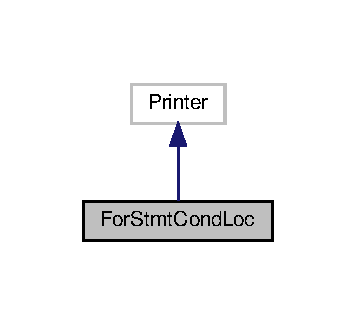
\includegraphics[width=171pt]{classForStmtCondLoc__inherit__graph}
\end{center}
\end{figure}


Collaboration diagram for For\+Stmt\+Cond\+Loc\+:\nopagebreak
\begin{figure}[H]
\begin{center}
\leavevmode
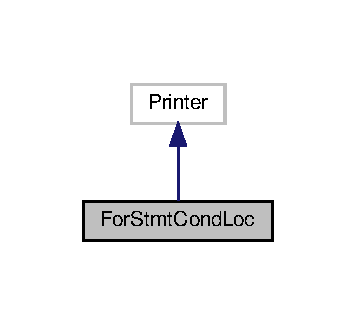
\includegraphics[width=171pt]{classForStmtCondLoc__coll__graph}
\end{center}
\end{figure}
\subsection*{Public Member Functions}
\begin{DoxyCompactItemize}
\item 
\hyperlink{classForStmtCondLoc_a62921ad2ca6417c087e8aa28395aee91}{For\+Stmt\+Cond\+Loc} ()
\item 
\hyperlink{classForStmtCondLoc_acb5c9643f2ce6be473e989c23c2d50e6}{For\+Stmt\+Cond\+Loc} (const \hyperlink{classForStmtCondLoc}{For\+Stmt\+Cond\+Loc} \&fscl)=delete
\item 
void \hyperlink{classForStmtCondLoc_a4579427843bc16d2ae834d234ed4a637}{get\+Cond\+Loc} (Expr $\ast$cond)
\item 
int \hyperlink{classForStmtCondLoc_adbb37a870f04545f48f62569b41f5102}{get\+Begin\+Line} ()
\item 
int \hyperlink{classForStmtCondLoc_a7db6511efc55de237119bc13f80915e0}{get\+Begin\+Col} ()
\item 
int \hyperlink{classForStmtCondLoc_aa3dc75623c0ccbc94fbd42ec784eeba1}{get\+End\+Line} ()
\item 
int \hyperlink{classForStmtCondLoc_a68dd344d53c30751ca6c0f6c4aaa49d0}{get\+End\+Col} ()
\end{DoxyCompactItemize}


\subsection{Detailed Description}
存储条件语句位置的类 

\subsection{Constructor \& Destructor Documentation}
\mbox{\Hypertarget{classForStmtCondLoc_a62921ad2ca6417c087e8aa28395aee91}\label{classForStmtCondLoc_a62921ad2ca6417c087e8aa28395aee91}} 
\index{For\+Stmt\+Cond\+Loc@{For\+Stmt\+Cond\+Loc}!For\+Stmt\+Cond\+Loc@{For\+Stmt\+Cond\+Loc}}
\index{For\+Stmt\+Cond\+Loc@{For\+Stmt\+Cond\+Loc}!For\+Stmt\+Cond\+Loc@{For\+Stmt\+Cond\+Loc}}
\subsubsection{\texorpdfstring{For\+Stmt\+Cond\+Loc()}{ForStmtCondLoc()}\hspace{0.1cm}{\footnotesize\ttfamily [1/2]}}
{\footnotesize\ttfamily For\+Stmt\+Cond\+Loc\+::\+For\+Stmt\+Cond\+Loc (\begin{DoxyParamCaption}{ }\end{DoxyParamCaption})}

构造函数 \mbox{\Hypertarget{classForStmtCondLoc_acb5c9643f2ce6be473e989c23c2d50e6}\label{classForStmtCondLoc_acb5c9643f2ce6be473e989c23c2d50e6}} 
\index{For\+Stmt\+Cond\+Loc@{For\+Stmt\+Cond\+Loc}!For\+Stmt\+Cond\+Loc@{For\+Stmt\+Cond\+Loc}}
\index{For\+Stmt\+Cond\+Loc@{For\+Stmt\+Cond\+Loc}!For\+Stmt\+Cond\+Loc@{For\+Stmt\+Cond\+Loc}}
\subsubsection{\texorpdfstring{For\+Stmt\+Cond\+Loc()}{ForStmtCondLoc()}\hspace{0.1cm}{\footnotesize\ttfamily [2/2]}}
{\footnotesize\ttfamily For\+Stmt\+Cond\+Loc\+::\+For\+Stmt\+Cond\+Loc (\begin{DoxyParamCaption}\item[{const \hyperlink{classForStmtCondLoc}{For\+Stmt\+Cond\+Loc} \&}]{fscl }\end{DoxyParamCaption})\hspace{0.3cm}{\ttfamily [delete]}}

拷贝构造函数(已禁用) 

\subsection{Member Function Documentation}
\mbox{\Hypertarget{classForStmtCondLoc_a7db6511efc55de237119bc13f80915e0}\label{classForStmtCondLoc_a7db6511efc55de237119bc13f80915e0}} 
\index{For\+Stmt\+Cond\+Loc@{For\+Stmt\+Cond\+Loc}!get\+Begin\+Col@{get\+Begin\+Col}}
\index{get\+Begin\+Col@{get\+Begin\+Col}!For\+Stmt\+Cond\+Loc@{For\+Stmt\+Cond\+Loc}}
\subsubsection{\texorpdfstring{get\+Begin\+Col()}{getBeginCol()}}
{\footnotesize\ttfamily int For\+Stmt\+Cond\+Loc\+::get\+Begin\+Col (\begin{DoxyParamCaption}{ }\end{DoxyParamCaption})}

返回条件语句的开始列

\begin{DoxyReturn}{Returns}
条件语句的开始列号 
\end{DoxyReturn}
\mbox{\Hypertarget{classForStmtCondLoc_adbb37a870f04545f48f62569b41f5102}\label{classForStmtCondLoc_adbb37a870f04545f48f62569b41f5102}} 
\index{For\+Stmt\+Cond\+Loc@{For\+Stmt\+Cond\+Loc}!get\+Begin\+Line@{get\+Begin\+Line}}
\index{get\+Begin\+Line@{get\+Begin\+Line}!For\+Stmt\+Cond\+Loc@{For\+Stmt\+Cond\+Loc}}
\subsubsection{\texorpdfstring{get\+Begin\+Line()}{getBeginLine()}}
{\footnotesize\ttfamily int For\+Stmt\+Cond\+Loc\+::get\+Begin\+Line (\begin{DoxyParamCaption}{ }\end{DoxyParamCaption})}

返回条件语句的开始行

\begin{DoxyReturn}{Returns}
条件语句的开始行号 
\end{DoxyReturn}
\mbox{\Hypertarget{classForStmtCondLoc_a4579427843bc16d2ae834d234ed4a637}\label{classForStmtCondLoc_a4579427843bc16d2ae834d234ed4a637}} 
\index{For\+Stmt\+Cond\+Loc@{For\+Stmt\+Cond\+Loc}!get\+Cond\+Loc@{get\+Cond\+Loc}}
\index{get\+Cond\+Loc@{get\+Cond\+Loc}!For\+Stmt\+Cond\+Loc@{For\+Stmt\+Cond\+Loc}}
\subsubsection{\texorpdfstring{get\+Cond\+Loc()}{getCondLoc()}}
{\footnotesize\ttfamily void For\+Stmt\+Cond\+Loc\+::get\+Cond\+Loc (\begin{DoxyParamCaption}\item[{Expr $\ast$}]{cond }\end{DoxyParamCaption})}

入口函数 寻找条件语句的各个位置 
\begin{DoxyParams}{Parameters}
{\em cond} & 获取到的条件语句\\
\hline
\end{DoxyParams}
寻找条件语句的位置信息 
\begin{DoxyParams}{Parameters}
{\em cond} & 循环的条件语句 \\
\hline
\end{DoxyParams}
\mbox{\Hypertarget{classForStmtCondLoc_a68dd344d53c30751ca6c0f6c4aaa49d0}\label{classForStmtCondLoc_a68dd344d53c30751ca6c0f6c4aaa49d0}} 
\index{For\+Stmt\+Cond\+Loc@{For\+Stmt\+Cond\+Loc}!get\+End\+Col@{get\+End\+Col}}
\index{get\+End\+Col@{get\+End\+Col}!For\+Stmt\+Cond\+Loc@{For\+Stmt\+Cond\+Loc}}
\subsubsection{\texorpdfstring{get\+End\+Col()}{getEndCol()}}
{\footnotesize\ttfamily int For\+Stmt\+Cond\+Loc\+::get\+End\+Col (\begin{DoxyParamCaption}{ }\end{DoxyParamCaption})}

返回条件语句的终结列

\begin{DoxyReturn}{Returns}
条件语句的结尾列号 
\end{DoxyReturn}
\mbox{\Hypertarget{classForStmtCondLoc_aa3dc75623c0ccbc94fbd42ec784eeba1}\label{classForStmtCondLoc_aa3dc75623c0ccbc94fbd42ec784eeba1}} 
\index{For\+Stmt\+Cond\+Loc@{For\+Stmt\+Cond\+Loc}!get\+End\+Line@{get\+End\+Line}}
\index{get\+End\+Line@{get\+End\+Line}!For\+Stmt\+Cond\+Loc@{For\+Stmt\+Cond\+Loc}}
\subsubsection{\texorpdfstring{get\+End\+Line()}{getEndLine()}}
{\footnotesize\ttfamily int For\+Stmt\+Cond\+Loc\+::get\+End\+Line (\begin{DoxyParamCaption}{ }\end{DoxyParamCaption})}

返回条件语句的终结行

\begin{DoxyReturn}{Returns}
条件语句的结尾行号 
\end{DoxyReturn}


The documentation for this class was generated from the following files\+:\begin{DoxyCompactItemize}
\item 
/mnt/hgfs/\+Git\+Hub/\+S\+Eexperiement/backend/\+A\+S\+T\+Visitor/src/\+Slow\+Memory\+Checker/\hyperlink{slowMemoryChecker_8h}{slow\+Memory\+Checker.\+h}\item 
/mnt/hgfs/\+Git\+Hub/\+S\+Eexperiement/backend/\+A\+S\+T\+Visitor/src/\+Slow\+Memory\+Checker/\hyperlink{slowMemoryChecker_8cpp}{slow\+Memory\+Checker.\+cpp}\end{DoxyCompactItemize}

\hypertarget{classReadConfig}{}\section{Read\+Config Class Reference}
\label{classReadConfig}\index{Read\+Config@{Read\+Config}}


{\ttfamily \#include $<$read\+Config.\+h$>$}

\subsection*{Public Member Functions}
\begin{DoxyCompactItemize}
\item 
char $\ast$ \hyperlink{classReadConfig_aa9e874be51af8937981d9e9c22339d39}{l\+\_\+trim} (char $\ast$sz\+Output, const char $\ast$sz\+Input)
\item 
char $\ast$ \hyperlink{classReadConfig_af726f6b598258c2672871fe720848327}{r\+\_\+trim} (char $\ast$sz\+Output, const char $\ast$sz\+Input)
\item 
char $\ast$ \hyperlink{classReadConfig_a2ad2a8fbfa2add5fa54fdfdae3953077}{a\+\_\+trim} (char $\ast$sz\+Output, const char $\ast$sz\+Input)
\item 
int \hyperlink{classReadConfig_aead8f510f2da60b56cbb0ec3f9f8bacb}{Get\+Profile\+String} (const char $\ast$profile, const char $\ast$App\+Name, const char $\ast$Key\+Name, char $\ast$Key\+Val)
\end{DoxyCompactItemize}


\subsection{Detailed Description}
读取配置文件的工具类 

\subsection{Member Function Documentation}
\mbox{\Hypertarget{classReadConfig_a2ad2a8fbfa2add5fa54fdfdae3953077}\label{classReadConfig_a2ad2a8fbfa2add5fa54fdfdae3953077}} 
\index{Read\+Config@{Read\+Config}!a\+\_\+trim@{a\+\_\+trim}}
\index{a\+\_\+trim@{a\+\_\+trim}!Read\+Config@{Read\+Config}}
\subsubsection{\texorpdfstring{a\+\_\+trim()}{a\_trim()}}
{\footnotesize\ttfamily char$\ast$ Read\+Config\+::a\+\_\+trim (\begin{DoxyParamCaption}\item[{char $\ast$}]{sz\+Output,  }\item[{const char $\ast$}]{sz\+Input }\end{DoxyParamCaption})\hspace{0.3cm}{\ttfamily [inline]}}

删除等号两边的空格 \mbox{\Hypertarget{classReadConfig_aead8f510f2da60b56cbb0ec3f9f8bacb}\label{classReadConfig_aead8f510f2da60b56cbb0ec3f9f8bacb}} 
\index{Read\+Config@{Read\+Config}!Get\+Profile\+String@{Get\+Profile\+String}}
\index{Get\+Profile\+String@{Get\+Profile\+String}!Read\+Config@{Read\+Config}}
\subsubsection{\texorpdfstring{Get\+Profile\+String()}{GetProfileString()}}
{\footnotesize\ttfamily int Read\+Config\+::\+Get\+Profile\+String (\begin{DoxyParamCaption}\item[{const char $\ast$}]{profile,  }\item[{const char $\ast$}]{App\+Name,  }\item[{const char $\ast$}]{Key\+Name,  }\item[{char $\ast$}]{Key\+Val }\end{DoxyParamCaption})\hspace{0.3cm}{\ttfamily [inline]}}

读取配置文件中的信息 
\begin{DoxyParams}{Parameters}
{\em profile} & 配置文件路径 \\
\hline
{\em App\+Name} & 模块名称 \\
\hline
{\em Key\+Name} & 变量的名称 \\
\hline
{\em Key\+Val} & 变量的值 \\
\hline
\end{DoxyParams}
\mbox{\Hypertarget{classReadConfig_aa9e874be51af8937981d9e9c22339d39}\label{classReadConfig_aa9e874be51af8937981d9e9c22339d39}} 
\index{Read\+Config@{Read\+Config}!l\+\_\+trim@{l\+\_\+trim}}
\index{l\+\_\+trim@{l\+\_\+trim}!Read\+Config@{Read\+Config}}
\subsubsection{\texorpdfstring{l\+\_\+trim()}{l\_trim()}}
{\footnotesize\ttfamily char$\ast$ Read\+Config\+::l\+\_\+trim (\begin{DoxyParamCaption}\item[{char $\ast$}]{sz\+Output,  }\item[{const char $\ast$}]{sz\+Input }\end{DoxyParamCaption})\hspace{0.3cm}{\ttfamily [inline]}}

删除左边的空格 \mbox{\Hypertarget{classReadConfig_af726f6b598258c2672871fe720848327}\label{classReadConfig_af726f6b598258c2672871fe720848327}} 
\index{Read\+Config@{Read\+Config}!r\+\_\+trim@{r\+\_\+trim}}
\index{r\+\_\+trim@{r\+\_\+trim}!Read\+Config@{Read\+Config}}
\subsubsection{\texorpdfstring{r\+\_\+trim()}{r\_trim()}}
{\footnotesize\ttfamily char$\ast$ Read\+Config\+::r\+\_\+trim (\begin{DoxyParamCaption}\item[{char $\ast$}]{sz\+Output,  }\item[{const char $\ast$}]{sz\+Input }\end{DoxyParamCaption})\hspace{0.3cm}{\ttfamily [inline]}}

删除右边的空格 

The documentation for this class was generated from the following file\+:\begin{DoxyCompactItemize}
\item 
/mnt/hgfs/\+Git\+Hub/\+S\+Eexperiement/backend/\+A\+S\+T\+Visitor/src/\+Slow\+Memory\+Checker/\hyperlink{readConfig_8h}{read\+Config.\+h}\end{DoxyCompactItemize}

\hypertarget{classSlowMemoryChecker}{}\section{Slow\+Memory\+Checker Class Reference}
\label{classSlowMemoryChecker}\index{Slow\+Memory\+Checker@{Slow\+Memory\+Checker}}


{\ttfamily \#include $<$slow\+Memory\+Checker.\+h$>$}



Inheritance diagram for Slow\+Memory\+Checker\+:\nopagebreak
\begin{figure}[H]
\begin{center}
\leavevmode
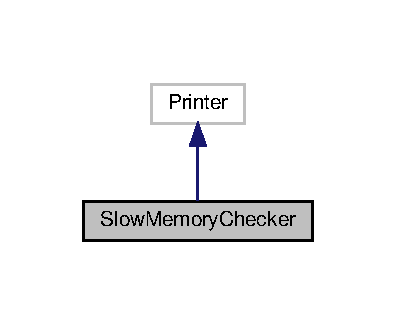
\includegraphics[width=190pt]{classSlowMemoryChecker__inherit__graph}
\end{center}
\end{figure}


Collaboration diagram for Slow\+Memory\+Checker\+:\nopagebreak
\begin{figure}[H]
\begin{center}
\leavevmode
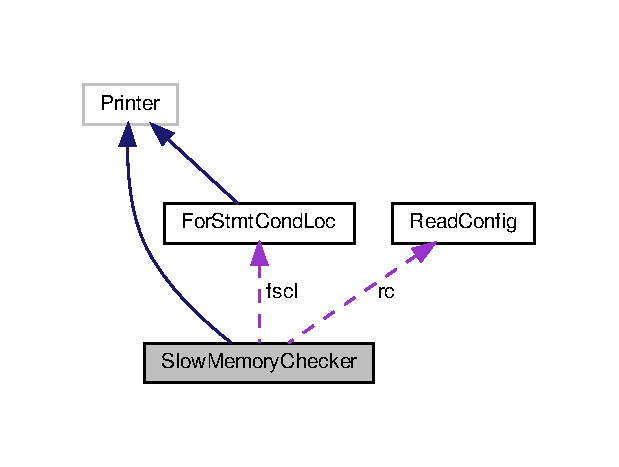
\includegraphics[width=297pt]{classSlowMemoryChecker__coll__graph}
\end{center}
\end{figure}
\subsection*{Public Member Functions}
\begin{DoxyCompactItemize}
\item 
\hyperlink{classSlowMemoryChecker_aafb7e74263259c4c229d369676711b96}{Slow\+Memory\+Checker} ()
\item 
\mbox{\Hypertarget{classSlowMemoryChecker_a6b14a889e02bdb4777b869ba0126c3f7}\label{classSlowMemoryChecker_a6b14a889e02bdb4777b869ba0126c3f7}} 
{\bfseries Slow\+Memory\+Checker} (const \hyperlink{classSlowMemoryChecker}{Slow\+Memory\+Checker} \&smc)=delete
\item 
void \hyperlink{classSlowMemoryChecker_addf5d951f4735a6a997dcf06a425192e}{Binary\+Operation\+Check} (Binary\+Operator $\ast$bo, int Binary\+Operator\+Line, int \hyperlink{classSlowMemoryChecker_a230d1bf30480bb33d1ed48e4f1e49074}{For\+Stmt\+End\+Line}, int \hyperlink{classSlowMemoryChecker_a71abe72c12d48e7763aaff2a2af2520d}{While\+Stmt\+End\+Line})
\item 
bool \hyperlink{classSlowMemoryChecker_a1be08d6dc0b018dae13f322237c876bf}{same\+Type} (Qual\+Type ltype, Qual\+Type rtype)
\item 
void \hyperlink{classSlowMemoryChecker_a8412000ccd35734216b9a1fc5b99de36}{print\+Call\+Expr\+Name} (clang\+::\+Call\+Expr $\ast$c)
\item 
void \hyperlink{classSlowMemoryChecker_aa931eca07137a39bcaa9f73008509fe5}{print\+C\+X\+X\+Call\+Expr\+Name} (C\+X\+X\+Operator\+Call\+Expr $\ast$c)
\item 
int \hyperlink{classSlowMemoryChecker_ab0d9194cf13d5a1419ca7b22c0c0d87b}{find\+While\+Stmt\+End\+Line} (While\+Stmt $\ast$ws)
\item 
int \hyperlink{classSlowMemoryChecker_ade0f9d36e7f56ab233ed85728fa414f7}{find\+For\+Stmt\+End\+Line} (For\+Stmt $\ast$fs)
\item 
int \hyperlink{classSlowMemoryChecker_a52801e0ccf9bf4bf9c92b2edee32b87d}{find\+Do\+While\+Stmt\+End\+Line} (Do\+Stmt $\ast$ds)
\item 
bool \hyperlink{classSlowMemoryChecker_a3100c7b5ee2060470b1626001b7cd2f0}{Find\+Expr\+Name\+By\+Token} (Expr $\ast$e)
\item 
bool \hyperlink{classSlowMemoryChecker_ab966e1b0878f20f8e0948026122949ee}{is\+Binary\+Oprator\+In\+Cond} (Binary\+Operator $\ast$bo)
\item 
bool \hyperlink{classSlowMemoryChecker_a33f70c0075e5258d7f0a9ee80e17aa51}{is\+Assignment\+Op\+In\+For\+Head} (Binary\+Operator $\ast$bo)
\item 
int \hyperlink{classSlowMemoryChecker_a0ab606cbdde59e08633052c1f14d9943}{get\+Num\+Of\+Loop} (Binary\+Operator $\ast$bo, int line, int col, int init\+Val)
\item 
bool \hyperlink{classSlowMemoryChecker_a0f71da7aae4b71c12a7b9d6b9bea38ee}{is\+Comparison\+Operator} (Binary\+Operator $\ast$bo)
\item 
int \hyperlink{classSlowMemoryChecker_a38de8a47b69ae3a78d731419aef3be0b}{get\+Init\+Val} (Binary\+Operator $\ast$bo)
\item 
bool \hyperlink{classSlowMemoryChecker_add99de7c17a94aaa19f4d3a73a3c54e3}{is\+Var\+Decl\+In\+For\+Head} (Var\+Decl $\ast$vd)
\item 
int \hyperlink{classSlowMemoryChecker_a6af096fd1aa1fdb3bedcf5a6909356e3}{get\+Init\+Val\+From\+Var\+Decl} (Var\+Decl $\ast$vd)
\item 
void \hyperlink{classSlowMemoryChecker_a0e208795d7bc6296d088333ae56f4b05}{Binary\+Operation\+Check\+In\+For\+Stmt} (Binary\+Operator $\ast$bo)
\item 
void \hyperlink{classSlowMemoryChecker_a0381c1159a96a8aa62ec77770d37a1e2}{Binary\+Operation\+Check\+In\+While\+Stmt} (Binary\+Operator $\ast$bo)
\item 
void \hyperlink{classSlowMemoryChecker_a15bcf8610e7d2c320e6f421cbaacb7a2}{Binary\+Operation\+Check\+In\+Do\+While\+Stmt} (Binary\+Operator $\ast$bo)
\item 
void \hyperlink{classSlowMemoryChecker_a5fa3e63b12a71fa0e9a01b2dd7fca80e}{set\+Flags} (Stmt $\ast$stmt)
\item 
int \hyperlink{classSlowMemoryChecker_a945d8af10cfed2f24e0ac9918d1b9594}{get\+Num\+Of\+Do\+While\+Loop} (int line, int col, int init\+Val)
\item 
void \hyperlink{classSlowMemoryChecker_a00c873c2d0209a6b94522162fac916ea}{debug} (const char $\ast$s)
\item 
bool \hyperlink{classSlowMemoryChecker_a0240abd96c40e96419ff7cb30b853ac4}{checke\+File\+Name} (Source\+Location begin\+Loc)
\end{DoxyCompactItemize}
\subsection*{Public Attributes}
\begin{DoxyCompactItemize}
\item 
\hyperlink{classForStmtCondLoc}{For\+Stmt\+Cond\+Loc} \hyperlink{classSlowMemoryChecker_ae82ceb324d6ca8eda59cafba44f0670e}{fscl}
\item 
Var\+Decl $\ast$ \hyperlink{classSlowMemoryChecker_a522a9d9f1e8cc77f3b60c0145b5f966b}{For\+Init\+Var\+Decl}
\item 
bool \hyperlink{classSlowMemoryChecker_afe1c220a2bf2af2ff289cd8d2034559f}{Var\+Decl\+In\+For\+Head}
\item 
int \hyperlink{classSlowMemoryChecker_a30178b54b18c14cf7f27e389885c92b1}{num\+Of\+For\+Loop}
\item 
int \hyperlink{classSlowMemoryChecker_a7ff6e854fe66a71e0f3cc2c9ee10612f}{num\+Of\+While\+Loop}
\item 
int \hyperlink{classSlowMemoryChecker_af3f2be4009f1b210d26a098b95b40494}{num\+Of\+Do\+While\+Loop}
\item 
int \hyperlink{classSlowMemoryChecker_a9152607c17f9a4200389de218a874889}{min\+Num\+Of\+Loop}
\item 
bool \hyperlink{classSlowMemoryChecker_a3eed183aed60d430815ff47d4a333eda}{in\+For\+Stmt}
\item 
int \hyperlink{classSlowMemoryChecker_a230d1bf30480bb33d1ed48e4f1e49074}{For\+Stmt\+End\+Line}
\item 
bool \hyperlink{classSlowMemoryChecker_ae644af0c0e0183c9eba51f406f7cc457}{in\+While\+Stmt}
\item 
int \hyperlink{classSlowMemoryChecker_a71abe72c12d48e7763aaff2a2af2520d}{While\+Stmt\+End\+Line}
\item 
bool \hyperlink{classSlowMemoryChecker_afb3646a2a66b2b5bb6830efec3455569}{in\+Do\+While\+Stmt}
\item 
int \hyperlink{classSlowMemoryChecker_aba744f1e41047a1df4d328fc8f683539}{Do\+While\+Stmt\+End\+Line}
\item 
Expr $\ast$ \hyperlink{classSlowMemoryChecker_a0e67ec70b12660a16935a9249cce7f26}{Do\+While\+Cond}
\item 
\hyperlink{classReadConfig}{Read\+Config} \hyperlink{classSlowMemoryChecker_a01724505f560bc3c1643881785254d67}{rc}
\end{DoxyCompactItemize}


\subsection{Detailed Description}
检测慢速内存操作的主类 

\subsection{Constructor \& Destructor Documentation}
\mbox{\Hypertarget{classSlowMemoryChecker_aafb7e74263259c4c229d369676711b96}\label{classSlowMemoryChecker_aafb7e74263259c4c229d369676711b96}} 
\index{Slow\+Memory\+Checker@{Slow\+Memory\+Checker}!Slow\+Memory\+Checker@{Slow\+Memory\+Checker}}
\index{Slow\+Memory\+Checker@{Slow\+Memory\+Checker}!Slow\+Memory\+Checker@{Slow\+Memory\+Checker}}
\subsubsection{\texorpdfstring{Slow\+Memory\+Checker()}{SlowMemoryChecker()}}
{\footnotesize\ttfamily Slow\+Memory\+Checker\+::\+Slow\+Memory\+Checker (\begin{DoxyParamCaption}{ }\end{DoxyParamCaption})}

构造函数 这里读取了配置文件中的最小循环次数(告警阈值) 如果读取配置文件错误,会将最小循环次数(告警阈值)设置为默认的1024 

\subsection{Member Function Documentation}
\mbox{\Hypertarget{classSlowMemoryChecker_addf5d951f4735a6a997dcf06a425192e}\label{classSlowMemoryChecker_addf5d951f4735a6a997dcf06a425192e}} 
\index{Slow\+Memory\+Checker@{Slow\+Memory\+Checker}!Binary\+Operation\+Check@{Binary\+Operation\+Check}}
\index{Binary\+Operation\+Check@{Binary\+Operation\+Check}!Slow\+Memory\+Checker@{Slow\+Memory\+Checker}}
\subsubsection{\texorpdfstring{Binary\+Operation\+Check()}{BinaryOperationCheck()}}
{\footnotesize\ttfamily void Slow\+Memory\+Checker\+::\+Binary\+Operation\+Check (\begin{DoxyParamCaption}\item[{Binary\+Operator $\ast$}]{bo,  }\item[{int}]{Binary\+Operator\+Line,  }\item[{int}]{For\+Stmt\+End\+Line,  }\item[{int}]{While\+Stmt\+End\+Line }\end{DoxyParamCaption})}

Slow\+Memory\+Checker的入口 从这里开始调用不同语句的\+Checke函数 
\begin{DoxyParams}{Parameters}
{\em bo} & 目前的操作符 \\
\hline
\end{DoxyParams}
\mbox{\Hypertarget{classSlowMemoryChecker_a15bcf8610e7d2c320e6f421cbaacb7a2}\label{classSlowMemoryChecker_a15bcf8610e7d2c320e6f421cbaacb7a2}} 
\index{Slow\+Memory\+Checker@{Slow\+Memory\+Checker}!Binary\+Operation\+Check\+In\+Do\+While\+Stmt@{Binary\+Operation\+Check\+In\+Do\+While\+Stmt}}
\index{Binary\+Operation\+Check\+In\+Do\+While\+Stmt@{Binary\+Operation\+Check\+In\+Do\+While\+Stmt}!Slow\+Memory\+Checker@{Slow\+Memory\+Checker}}
\subsubsection{\texorpdfstring{Binary\+Operation\+Check\+In\+Do\+While\+Stmt()}{BinaryOperationCheckInDoWhileStmt()}}
{\footnotesize\ttfamily void Slow\+Memory\+Checker\+::\+Binary\+Operation\+Check\+In\+Do\+While\+Stmt (\begin{DoxyParamCaption}\item[{Binary\+Operator $\ast$}]{bo }\end{DoxyParamCaption})}

Do\+While语句的判断函数 其中默认循环变量初值为零 根据推算的循环次数以及变量大小决定是否告警 
\begin{DoxyParams}{Parameters}
{\em bo} & 目前的操作符 \\
\hline
\end{DoxyParams}
\mbox{\Hypertarget{classSlowMemoryChecker_a0e208795d7bc6296d088333ae56f4b05}\label{classSlowMemoryChecker_a0e208795d7bc6296d088333ae56f4b05}} 
\index{Slow\+Memory\+Checker@{Slow\+Memory\+Checker}!Binary\+Operation\+Check\+In\+For\+Stmt@{Binary\+Operation\+Check\+In\+For\+Stmt}}
\index{Binary\+Operation\+Check\+In\+For\+Stmt@{Binary\+Operation\+Check\+In\+For\+Stmt}!Slow\+Memory\+Checker@{Slow\+Memory\+Checker}}
\subsubsection{\texorpdfstring{Binary\+Operation\+Check\+In\+For\+Stmt()}{BinaryOperationCheckInForStmt()}}
{\footnotesize\ttfamily void Slow\+Memory\+Checker\+::\+Binary\+Operation\+Check\+In\+For\+Stmt (\begin{DoxyParamCaption}\item[{Binary\+Operator $\ast$}]{bo }\end{DoxyParamCaption})}

For语句的判断函数 根据for语句头获取循环变量初值 根据推算的循环次数以及变量大小决定是否告警 
\begin{DoxyParams}{Parameters}
{\em bo} & 目前的操作符 \\
\hline
\end{DoxyParams}
\mbox{\Hypertarget{classSlowMemoryChecker_a0381c1159a96a8aa62ec77770d37a1e2}\label{classSlowMemoryChecker_a0381c1159a96a8aa62ec77770d37a1e2}} 
\index{Slow\+Memory\+Checker@{Slow\+Memory\+Checker}!Binary\+Operation\+Check\+In\+While\+Stmt@{Binary\+Operation\+Check\+In\+While\+Stmt}}
\index{Binary\+Operation\+Check\+In\+While\+Stmt@{Binary\+Operation\+Check\+In\+While\+Stmt}!Slow\+Memory\+Checker@{Slow\+Memory\+Checker}}
\subsubsection{\texorpdfstring{Binary\+Operation\+Check\+In\+While\+Stmt()}{BinaryOperationCheckInWhileStmt()}}
{\footnotesize\ttfamily void Slow\+Memory\+Checker\+::\+Binary\+Operation\+Check\+In\+While\+Stmt (\begin{DoxyParamCaption}\item[{Binary\+Operator $\ast$}]{bo }\end{DoxyParamCaption})}

While语句的判断函数 其中默认循环变量初值为零 根据推算的循环次数以及变量大小决定是否告警 
\begin{DoxyParams}{Parameters}
{\em bo} & 目前的操作符 \\
\hline
\end{DoxyParams}
\mbox{\Hypertarget{classSlowMemoryChecker_a0240abd96c40e96419ff7cb30b853ac4}\label{classSlowMemoryChecker_a0240abd96c40e96419ff7cb30b853ac4}} 
\index{Slow\+Memory\+Checker@{Slow\+Memory\+Checker}!checke\+File\+Name@{checke\+File\+Name}}
\index{checke\+File\+Name@{checke\+File\+Name}!Slow\+Memory\+Checker@{Slow\+Memory\+Checker}}
\subsubsection{\texorpdfstring{checke\+File\+Name()}{checkeFileName()}}
{\footnotesize\ttfamily bool Slow\+Memory\+Checker\+::checke\+File\+Name (\begin{DoxyParamCaption}\item[{Source\+Location}]{begin\+Loc }\end{DoxyParamCaption})}

根据单元位置获取目前的文件信息 用以区分无需分析的头文件以及需要分析的源文件 
\begin{DoxyParams}{Parameters}
{\em begin\+Loc} & 目前的单元开始位置 \\
\hline
\end{DoxyParams}

\begin{DoxyRetVals}{Return values}
{\em true} & 目前分析的文件是源文件 \\
\hline
{\em false} & 目前分析的文件是头文件或其他文件 \\
\hline
\end{DoxyRetVals}
\mbox{\Hypertarget{classSlowMemoryChecker_a00c873c2d0209a6b94522162fac916ea}\label{classSlowMemoryChecker_a00c873c2d0209a6b94522162fac916ea}} 
\index{Slow\+Memory\+Checker@{Slow\+Memory\+Checker}!debug@{debug}}
\index{debug@{debug}!Slow\+Memory\+Checker@{Slow\+Memory\+Checker}}
\subsubsection{\texorpdfstring{debug()}{debug()}}
{\footnotesize\ttfamily void Slow\+Memory\+Checker\+::debug (\begin{DoxyParamCaption}\item[{const char $\ast$}]{s }\end{DoxyParamCaption})}

debug 
\begin{DoxyParams}{Parameters}
{\em s} & 输出至控制台的字符串 \\
\hline
\end{DoxyParams}
\mbox{\Hypertarget{classSlowMemoryChecker_a52801e0ccf9bf4bf9c92b2edee32b87d}\label{classSlowMemoryChecker_a52801e0ccf9bf4bf9c92b2edee32b87d}} 
\index{Slow\+Memory\+Checker@{Slow\+Memory\+Checker}!find\+Do\+While\+Stmt\+End\+Line@{find\+Do\+While\+Stmt\+End\+Line}}
\index{find\+Do\+While\+Stmt\+End\+Line@{find\+Do\+While\+Stmt\+End\+Line}!Slow\+Memory\+Checker@{Slow\+Memory\+Checker}}
\subsubsection{\texorpdfstring{find\+Do\+While\+Stmt\+End\+Line()}{findDoWhileStmtEndLine()}}
{\footnotesize\ttfamily int Slow\+Memory\+Checker\+::find\+Do\+While\+Stmt\+End\+Line (\begin{DoxyParamCaption}\item[{Do\+Stmt $\ast$}]{ds }\end{DoxyParamCaption})}

找到\+Do\+While语句的结尾行号 用来判断之后的语句类型 
\begin{DoxyParams}{Parameters}
{\em ds} & 目前的\+Do\+While语句 \\
\hline
\end{DoxyParams}
\begin{DoxyReturn}{Returns}
Do\+While\+Stmt\+End\+Line 最近的\+Do\+While语句的结尾行号 
\end{DoxyReturn}
\mbox{\Hypertarget{classSlowMemoryChecker_a3100c7b5ee2060470b1626001b7cd2f0}\label{classSlowMemoryChecker_a3100c7b5ee2060470b1626001b7cd2f0}} 
\index{Slow\+Memory\+Checker@{Slow\+Memory\+Checker}!Find\+Expr\+Name\+By\+Token@{Find\+Expr\+Name\+By\+Token}}
\index{Find\+Expr\+Name\+By\+Token@{Find\+Expr\+Name\+By\+Token}!Slow\+Memory\+Checker@{Slow\+Memory\+Checker}}
\subsubsection{\texorpdfstring{Find\+Expr\+Name\+By\+Token()}{FindExprNameByToken()}}
{\footnotesize\ttfamily bool Slow\+Memory\+Checker\+::\+Find\+Expr\+Name\+By\+Token (\begin{DoxyParamCaption}\item[{Expr $\ast$}]{e }\end{DoxyParamCaption})}

使用token流寻找表达式的名字 测试用 \mbox{\Hypertarget{classSlowMemoryChecker_ade0f9d36e7f56ab233ed85728fa414f7}\label{classSlowMemoryChecker_ade0f9d36e7f56ab233ed85728fa414f7}} 
\index{Slow\+Memory\+Checker@{Slow\+Memory\+Checker}!find\+For\+Stmt\+End\+Line@{find\+For\+Stmt\+End\+Line}}
\index{find\+For\+Stmt\+End\+Line@{find\+For\+Stmt\+End\+Line}!Slow\+Memory\+Checker@{Slow\+Memory\+Checker}}
\subsubsection{\texorpdfstring{find\+For\+Stmt\+End\+Line()}{findForStmtEndLine()}}
{\footnotesize\ttfamily int Slow\+Memory\+Checker\+::find\+For\+Stmt\+End\+Line (\begin{DoxyParamCaption}\item[{For\+Stmt $\ast$}]{fs }\end{DoxyParamCaption})}

找到\+For语句的结尾行号 用来判断之后的语句类型 
\begin{DoxyParams}{Parameters}
{\em fs} & 目前的\+For语句 \\
\hline
\end{DoxyParams}
\begin{DoxyReturn}{Returns}
For\+Stmt\+End\+Line 最近的\+For语句的结尾行号 
\end{DoxyReturn}
\mbox{\Hypertarget{classSlowMemoryChecker_ab0d9194cf13d5a1419ca7b22c0c0d87b}\label{classSlowMemoryChecker_ab0d9194cf13d5a1419ca7b22c0c0d87b}} 
\index{Slow\+Memory\+Checker@{Slow\+Memory\+Checker}!find\+While\+Stmt\+End\+Line@{find\+While\+Stmt\+End\+Line}}
\index{find\+While\+Stmt\+End\+Line@{find\+While\+Stmt\+End\+Line}!Slow\+Memory\+Checker@{Slow\+Memory\+Checker}}
\subsubsection{\texorpdfstring{find\+While\+Stmt\+End\+Line()}{findWhileStmtEndLine()}}
{\footnotesize\ttfamily int Slow\+Memory\+Checker\+::find\+While\+Stmt\+End\+Line (\begin{DoxyParamCaption}\item[{While\+Stmt $\ast$}]{ws }\end{DoxyParamCaption})}

找到\+While语句的结尾行号 用来判断之后的语句类型 
\begin{DoxyParams}{Parameters}
{\em ws} & 目前的\+While语句 \\
\hline
\end{DoxyParams}
\begin{DoxyReturn}{Returns}
While\+Stmt\+End\+Line 最近的\+While语句的结尾行号 
\end{DoxyReturn}
\mbox{\Hypertarget{classSlowMemoryChecker_a38de8a47b69ae3a78d731419aef3be0b}\label{classSlowMemoryChecker_a38de8a47b69ae3a78d731419aef3be0b}} 
\index{Slow\+Memory\+Checker@{Slow\+Memory\+Checker}!get\+Init\+Val@{get\+Init\+Val}}
\index{get\+Init\+Val@{get\+Init\+Val}!Slow\+Memory\+Checker@{Slow\+Memory\+Checker}}
\subsubsection{\texorpdfstring{get\+Init\+Val()}{getInitVal()}}
{\footnotesize\ttfamily int Slow\+Memory\+Checker\+::get\+Init\+Val (\begin{DoxyParamCaption}\item[{Binary\+Operator $\ast$}]{bo }\end{DoxyParamCaption})}

根据目前的操作符 获取\+For语句的循环变量的初始值 在\+Binary\+Operation\+Check\+In\+For\+Stmt中被调用 (\+For语句头部中有赋值语句的情况被调用) 
\begin{DoxyParams}{Parameters}
{\em bo} & 目前的二元操作符 \\
\hline
\end{DoxyParams}
\begin{DoxyReturn}{Returns}
val For语句的循环变量的初始值 
\end{DoxyReturn}
\mbox{\Hypertarget{classSlowMemoryChecker_a6af096fd1aa1fdb3bedcf5a6909356e3}\label{classSlowMemoryChecker_a6af096fd1aa1fdb3bedcf5a6909356e3}} 
\index{Slow\+Memory\+Checker@{Slow\+Memory\+Checker}!get\+Init\+Val\+From\+Var\+Decl@{get\+Init\+Val\+From\+Var\+Decl}}
\index{get\+Init\+Val\+From\+Var\+Decl@{get\+Init\+Val\+From\+Var\+Decl}!Slow\+Memory\+Checker@{Slow\+Memory\+Checker}}
\subsubsection{\texorpdfstring{get\+Init\+Val\+From\+Var\+Decl()}{getInitValFromVarDecl()}}
{\footnotesize\ttfamily int Slow\+Memory\+Checker\+::get\+Init\+Val\+From\+Var\+Decl (\begin{DoxyParamCaption}\item[{Var\+Decl $\ast$}]{vd }\end{DoxyParamCaption})}

根据目前的声明语句 获取\+For语句的循环变量的初始值 在\+Binary\+Operation\+Check\+In\+For\+Stmt中被调用 (\+For语句头部中有声明语句的情况被调用) 
\begin{DoxyParams}{Parameters}
{\em vd} & 目前的声明语句 \\
\hline
\end{DoxyParams}
\begin{DoxyReturn}{Returns}
val For语句的循环变量的初始值 
\end{DoxyReturn}
\mbox{\Hypertarget{classSlowMemoryChecker_a945d8af10cfed2f24e0ac9918d1b9594}\label{classSlowMemoryChecker_a945d8af10cfed2f24e0ac9918d1b9594}} 
\index{Slow\+Memory\+Checker@{Slow\+Memory\+Checker}!get\+Num\+Of\+Do\+While\+Loop@{get\+Num\+Of\+Do\+While\+Loop}}
\index{get\+Num\+Of\+Do\+While\+Loop@{get\+Num\+Of\+Do\+While\+Loop}!Slow\+Memory\+Checker@{Slow\+Memory\+Checker}}
\subsubsection{\texorpdfstring{get\+Num\+Of\+Do\+While\+Loop()}{getNumOfDoWhileLoop()}}
{\footnotesize\ttfamily int Slow\+Memory\+Checker\+::get\+Num\+Of\+Do\+While\+Loop (\begin{DoxyParamCaption}\item[{int}]{line,  }\item[{int}]{col,  }\item[{int}]{init\+Val }\end{DoxyParamCaption})}

根据目前的操作符 获取\+For语句的循环变量的初始值 在\+Binary\+Operation\+Check\+In\+For\+Stmt中被调用 (\+For语句头部中有赋值语句的情况被调用) 
\begin{DoxyParams}{Parameters}
{\em bo} & 目前的二元操作符 \\
\hline
\end{DoxyParams}
\begin{DoxyReturn}{Returns}
num\+Of\+Loop Do\+While语句的循环次数 
\end{DoxyReturn}
\mbox{\Hypertarget{classSlowMemoryChecker_a0ab606cbdde59e08633052c1f14d9943}\label{classSlowMemoryChecker_a0ab606cbdde59e08633052c1f14d9943}} 
\index{Slow\+Memory\+Checker@{Slow\+Memory\+Checker}!get\+Num\+Of\+Loop@{get\+Num\+Of\+Loop}}
\index{get\+Num\+Of\+Loop@{get\+Num\+Of\+Loop}!Slow\+Memory\+Checker@{Slow\+Memory\+Checker}}
\subsubsection{\texorpdfstring{get\+Num\+Of\+Loop()}{getNumOfLoop()}}
{\footnotesize\ttfamily int Slow\+Memory\+Checker\+::get\+Num\+Of\+Loop (\begin{DoxyParamCaption}\item[{Binary\+Operator $\ast$}]{bo,  }\item[{int}]{line,  }\item[{int}]{col,  }\item[{int}]{init\+Val }\end{DoxyParamCaption})}

根据目前的操作符以及循环变量初始值 尝试获取\+For语句的循环次数 在\+Binary\+Operation\+Check\+In\+For\+Stmt中被调用 
\begin{DoxyParams}{Parameters}
{\em bo} & 目前的二元操作符 \\
\hline
{\em init\+Val} & 循环变量初始值 \\
\hline
\end{DoxyParams}
\begin{DoxyReturn}{Returns}
num\+Of\+Loop For语句和\+While语句的循环次数 
\end{DoxyReturn}
\mbox{\Hypertarget{classSlowMemoryChecker_a33f70c0075e5258d7f0a9ee80e17aa51}\label{classSlowMemoryChecker_a33f70c0075e5258d7f0a9ee80e17aa51}} 
\index{Slow\+Memory\+Checker@{Slow\+Memory\+Checker}!is\+Assignment\+Op\+In\+For\+Head@{is\+Assignment\+Op\+In\+For\+Head}}
\index{is\+Assignment\+Op\+In\+For\+Head@{is\+Assignment\+Op\+In\+For\+Head}!Slow\+Memory\+Checker@{Slow\+Memory\+Checker}}
\subsubsection{\texorpdfstring{is\+Assignment\+Op\+In\+For\+Head()}{isAssignmentOpInForHead()}}
{\footnotesize\ttfamily bool Slow\+Memory\+Checker\+::is\+Assignment\+Op\+In\+For\+Head (\begin{DoxyParamCaption}\item[{Binary\+Operator $\ast$}]{bo }\end{DoxyParamCaption})}

判断赋值语句是否在\+For语句头部 
\begin{DoxyParams}{Parameters}
{\em bo} & 目前二元操作符(赋值) \\
\hline
\end{DoxyParams}

\begin{DoxyRetVals}{Return values}
{\em true} & 该赋值语句在\+For语句头部 \\
\hline
{\em false} & 该赋值语句不在\+For语句头部 \\
\hline
\end{DoxyRetVals}
\mbox{\Hypertarget{classSlowMemoryChecker_ab966e1b0878f20f8e0948026122949ee}\label{classSlowMemoryChecker_ab966e1b0878f20f8e0948026122949ee}} 
\index{Slow\+Memory\+Checker@{Slow\+Memory\+Checker}!is\+Binary\+Oprator\+In\+Cond@{is\+Binary\+Oprator\+In\+Cond}}
\index{is\+Binary\+Oprator\+In\+Cond@{is\+Binary\+Oprator\+In\+Cond}!Slow\+Memory\+Checker@{Slow\+Memory\+Checker}}
\subsubsection{\texorpdfstring{is\+Binary\+Oprator\+In\+Cond()}{isBinaryOpratorInCond()}}
{\footnotesize\ttfamily bool Slow\+Memory\+Checker\+::is\+Binary\+Oprator\+In\+Cond (\begin{DoxyParamCaption}\item[{Binary\+Operator $\ast$}]{bo }\end{DoxyParamCaption})}

判断操作符是否在循环的条件语句中 
\begin{DoxyParams}{Parameters}
{\em bo} & 目前二元操作符 \\
\hline
\end{DoxyParams}

\begin{DoxyRetVals}{Return values}
{\em true} & 操作符在循环的条件语句中 \\
\hline
{\em false} & 操作符不在循环的条件语句中 \\
\hline
\end{DoxyRetVals}
\mbox{\Hypertarget{classSlowMemoryChecker_a0f71da7aae4b71c12a7b9d6b9bea38ee}\label{classSlowMemoryChecker_a0f71da7aae4b71c12a7b9d6b9bea38ee}} 
\index{Slow\+Memory\+Checker@{Slow\+Memory\+Checker}!is\+Comparison\+Operator@{is\+Comparison\+Operator}}
\index{is\+Comparison\+Operator@{is\+Comparison\+Operator}!Slow\+Memory\+Checker@{Slow\+Memory\+Checker}}
\subsubsection{\texorpdfstring{is\+Comparison\+Operator()}{isComparisonOperator()}}
{\footnotesize\ttfamily bool Slow\+Memory\+Checker\+::is\+Comparison\+Operator (\begin{DoxyParamCaption}\item[{Binary\+Operator $\ast$}]{bo }\end{DoxyParamCaption})}

判断目前的二元操作符是否是比较操作符 
\begin{DoxyParams}{Parameters}
{\em bo} & 目前的二元操作符 \\
\hline
\end{DoxyParams}

\begin{DoxyRetVals}{Return values}
{\em true} & 目前的二元操作符是比较操作符 \\
\hline
{\em false} & 目前的二元操作符不是比较操作符 \\
\hline
\end{DoxyRetVals}
\mbox{\Hypertarget{classSlowMemoryChecker_add99de7c17a94aaa19f4d3a73a3c54e3}\label{classSlowMemoryChecker_add99de7c17a94aaa19f4d3a73a3c54e3}} 
\index{Slow\+Memory\+Checker@{Slow\+Memory\+Checker}!is\+Var\+Decl\+In\+For\+Head@{is\+Var\+Decl\+In\+For\+Head}}
\index{is\+Var\+Decl\+In\+For\+Head@{is\+Var\+Decl\+In\+For\+Head}!Slow\+Memory\+Checker@{Slow\+Memory\+Checker}}
\subsubsection{\texorpdfstring{is\+Var\+Decl\+In\+For\+Head()}{isVarDeclInForHead()}}
{\footnotesize\ttfamily bool Slow\+Memory\+Checker\+::is\+Var\+Decl\+In\+For\+Head (\begin{DoxyParamCaption}\item[{Var\+Decl $\ast$}]{vd }\end{DoxyParamCaption})}

根据\+For语句的条件语句 判断声明语句是否在\+For语句的头部 
\begin{DoxyParams}{Parameters}
{\em vd} & 目前的声明语句 \\
\hline
\end{DoxyParams}

\begin{DoxyRetVals}{Return values}
{\em true} & 语句在\+For语句的初始化语句中 \\
\hline
{\em false} & 语句不在\+For语句的初始化语句中 \\
\hline
\end{DoxyRetVals}
\mbox{\Hypertarget{classSlowMemoryChecker_a8412000ccd35734216b9a1fc5b99de36}\label{classSlowMemoryChecker_a8412000ccd35734216b9a1fc5b99de36}} 
\index{Slow\+Memory\+Checker@{Slow\+Memory\+Checker}!print\+Call\+Expr\+Name@{print\+Call\+Expr\+Name}}
\index{print\+Call\+Expr\+Name@{print\+Call\+Expr\+Name}!Slow\+Memory\+Checker@{Slow\+Memory\+Checker}}
\subsubsection{\texorpdfstring{print\+Call\+Expr\+Name()}{printCallExprName()}}
{\footnotesize\ttfamily void Slow\+Memory\+Checker\+::print\+Call\+Expr\+Name (\begin{DoxyParamCaption}\item[{clang\+::\+Call\+Expr $\ast$}]{c }\end{DoxyParamCaption})}

打印目前的调用函数名称 测试用 \mbox{\Hypertarget{classSlowMemoryChecker_aa931eca07137a39bcaa9f73008509fe5}\label{classSlowMemoryChecker_aa931eca07137a39bcaa9f73008509fe5}} 
\index{Slow\+Memory\+Checker@{Slow\+Memory\+Checker}!print\+C\+X\+X\+Call\+Expr\+Name@{print\+C\+X\+X\+Call\+Expr\+Name}}
\index{print\+C\+X\+X\+Call\+Expr\+Name@{print\+C\+X\+X\+Call\+Expr\+Name}!Slow\+Memory\+Checker@{Slow\+Memory\+Checker}}
\subsubsection{\texorpdfstring{print\+C\+X\+X\+Call\+Expr\+Name()}{printCXXCallExprName()}}
{\footnotesize\ttfamily void Slow\+Memory\+Checker\+::print\+C\+X\+X\+Call\+Expr\+Name (\begin{DoxyParamCaption}\item[{C\+X\+X\+Operator\+Call\+Expr $\ast$}]{c }\end{DoxyParamCaption})}

打印目前的调用函数名称 测试用 \mbox{\Hypertarget{classSlowMemoryChecker_a1be08d6dc0b018dae13f322237c876bf}\label{classSlowMemoryChecker_a1be08d6dc0b018dae13f322237c876bf}} 
\index{Slow\+Memory\+Checker@{Slow\+Memory\+Checker}!same\+Type@{same\+Type}}
\index{same\+Type@{same\+Type}!Slow\+Memory\+Checker@{Slow\+Memory\+Checker}}
\subsubsection{\texorpdfstring{same\+Type()}{sameType()}}
{\footnotesize\ttfamily bool Slow\+Memory\+Checker\+::same\+Type (\begin{DoxyParamCaption}\item[{Qual\+Type}]{ltype,  }\item[{Qual\+Type}]{rtype }\end{DoxyParamCaption})}

判断两个类型是否一致 
\begin{DoxyParams}{Parameters}
{\em ltype} & 类型一 \\
\hline
{\em rtype} & 类型二 \\
\hline
\end{DoxyParams}

\begin{DoxyRetVals}{Return values}
{\em true} & 两个类型一致 \\
\hline
{\em false} & 两个类型不一致 \\
\hline
\end{DoxyRetVals}
\mbox{\Hypertarget{classSlowMemoryChecker_a5fa3e63b12a71fa0e9a01b2dd7fca80e}\label{classSlowMemoryChecker_a5fa3e63b12a71fa0e9a01b2dd7fca80e}} 
\index{Slow\+Memory\+Checker@{Slow\+Memory\+Checker}!set\+Flags@{set\+Flags}}
\index{set\+Flags@{set\+Flags}!Slow\+Memory\+Checker@{Slow\+Memory\+Checker}}
\subsubsection{\texorpdfstring{set\+Flags()}{setFlags()}}
{\footnotesize\ttfamily void Slow\+Memory\+Checker\+::set\+Flags (\begin{DoxyParamCaption}\item[{Stmt $\ast$}]{s }\end{DoxyParamCaption})}

在visit\+Stmt中调用 主要功能是判断目前所在的语句类型 并且更新\+Checker所需的变量值 
\begin{DoxyParams}{Parameters}
{\em s} & 目前的语句 \\
\hline
\end{DoxyParams}


\subsection{Member Data Documentation}
\mbox{\Hypertarget{classSlowMemoryChecker_a0e67ec70b12660a16935a9249cce7f26}\label{classSlowMemoryChecker_a0e67ec70b12660a16935a9249cce7f26}} 
\index{Slow\+Memory\+Checker@{Slow\+Memory\+Checker}!Do\+While\+Cond@{Do\+While\+Cond}}
\index{Do\+While\+Cond@{Do\+While\+Cond}!Slow\+Memory\+Checker@{Slow\+Memory\+Checker}}
\subsubsection{\texorpdfstring{Do\+While\+Cond}{DoWhileCond}}
{\footnotesize\ttfamily Expr$\ast$ Slow\+Memory\+Checker\+::\+Do\+While\+Cond}

Do\+While语句的条件语句 因为在语句最后 特殊处理 \mbox{\Hypertarget{classSlowMemoryChecker_aba744f1e41047a1df4d328fc8f683539}\label{classSlowMemoryChecker_aba744f1e41047a1df4d328fc8f683539}} 
\index{Slow\+Memory\+Checker@{Slow\+Memory\+Checker}!Do\+While\+Stmt\+End\+Line@{Do\+While\+Stmt\+End\+Line}}
\index{Do\+While\+Stmt\+End\+Line@{Do\+While\+Stmt\+End\+Line}!Slow\+Memory\+Checker@{Slow\+Memory\+Checker}}
\subsubsection{\texorpdfstring{Do\+While\+Stmt\+End\+Line}{DoWhileStmtEndLine}}
{\footnotesize\ttfamily int Slow\+Memory\+Checker\+::\+Do\+While\+Stmt\+End\+Line}

最近的\+Do\+While循环终结行号 \mbox{\Hypertarget{classSlowMemoryChecker_a522a9d9f1e8cc77f3b60c0145b5f966b}\label{classSlowMemoryChecker_a522a9d9f1e8cc77f3b60c0145b5f966b}} 
\index{Slow\+Memory\+Checker@{Slow\+Memory\+Checker}!For\+Init\+Var\+Decl@{For\+Init\+Var\+Decl}}
\index{For\+Init\+Var\+Decl@{For\+Init\+Var\+Decl}!Slow\+Memory\+Checker@{Slow\+Memory\+Checker}}
\subsubsection{\texorpdfstring{For\+Init\+Var\+Decl}{ForInitVarDecl}}
{\footnotesize\ttfamily Var\+Decl$\ast$ Slow\+Memory\+Checker\+::\+For\+Init\+Var\+Decl}

For语句初始化中的变量声明语句 \mbox{\Hypertarget{classSlowMemoryChecker_a230d1bf30480bb33d1ed48e4f1e49074}\label{classSlowMemoryChecker_a230d1bf30480bb33d1ed48e4f1e49074}} 
\index{Slow\+Memory\+Checker@{Slow\+Memory\+Checker}!For\+Stmt\+End\+Line@{For\+Stmt\+End\+Line}}
\index{For\+Stmt\+End\+Line@{For\+Stmt\+End\+Line}!Slow\+Memory\+Checker@{Slow\+Memory\+Checker}}
\subsubsection{\texorpdfstring{For\+Stmt\+End\+Line}{ForStmtEndLine}}
{\footnotesize\ttfamily int Slow\+Memory\+Checker\+::\+For\+Stmt\+End\+Line}

最近的\+For循环终结行号 \mbox{\Hypertarget{classSlowMemoryChecker_ae82ceb324d6ca8eda59cafba44f0670e}\label{classSlowMemoryChecker_ae82ceb324d6ca8eda59cafba44f0670e}} 
\index{Slow\+Memory\+Checker@{Slow\+Memory\+Checker}!fscl@{fscl}}
\index{fscl@{fscl}!Slow\+Memory\+Checker@{Slow\+Memory\+Checker}}
\subsubsection{\texorpdfstring{fscl}{fscl}}
{\footnotesize\ttfamily \hyperlink{classForStmtCondLoc}{For\+Stmt\+Cond\+Loc} Slow\+Memory\+Checker\+::fscl}

最近遍历的条件语句 \mbox{\Hypertarget{classSlowMemoryChecker_afb3646a2a66b2b5bb6830efec3455569}\label{classSlowMemoryChecker_afb3646a2a66b2b5bb6830efec3455569}} 
\index{Slow\+Memory\+Checker@{Slow\+Memory\+Checker}!in\+Do\+While\+Stmt@{in\+Do\+While\+Stmt}}
\index{in\+Do\+While\+Stmt@{in\+Do\+While\+Stmt}!Slow\+Memory\+Checker@{Slow\+Memory\+Checker}}
\subsubsection{\texorpdfstring{in\+Do\+While\+Stmt}{inDoWhileStmt}}
{\footnotesize\ttfamily bool Slow\+Memory\+Checker\+::in\+Do\+While\+Stmt}

标示目前语句是否在\+Do\+While循环中 \mbox{\Hypertarget{classSlowMemoryChecker_a3eed183aed60d430815ff47d4a333eda}\label{classSlowMemoryChecker_a3eed183aed60d430815ff47d4a333eda}} 
\index{Slow\+Memory\+Checker@{Slow\+Memory\+Checker}!in\+For\+Stmt@{in\+For\+Stmt}}
\index{in\+For\+Stmt@{in\+For\+Stmt}!Slow\+Memory\+Checker@{Slow\+Memory\+Checker}}
\subsubsection{\texorpdfstring{in\+For\+Stmt}{inForStmt}}
{\footnotesize\ttfamily bool Slow\+Memory\+Checker\+::in\+For\+Stmt}

标示目前语句是否在\+For循环中 \mbox{\Hypertarget{classSlowMemoryChecker_ae644af0c0e0183c9eba51f406f7cc457}\label{classSlowMemoryChecker_ae644af0c0e0183c9eba51f406f7cc457}} 
\index{Slow\+Memory\+Checker@{Slow\+Memory\+Checker}!in\+While\+Stmt@{in\+While\+Stmt}}
\index{in\+While\+Stmt@{in\+While\+Stmt}!Slow\+Memory\+Checker@{Slow\+Memory\+Checker}}
\subsubsection{\texorpdfstring{in\+While\+Stmt}{inWhileStmt}}
{\footnotesize\ttfamily bool Slow\+Memory\+Checker\+::in\+While\+Stmt}

标示目前语句是否在\+While循环中 \mbox{\Hypertarget{classSlowMemoryChecker_a9152607c17f9a4200389de218a874889}\label{classSlowMemoryChecker_a9152607c17f9a4200389de218a874889}} 
\index{Slow\+Memory\+Checker@{Slow\+Memory\+Checker}!min\+Num\+Of\+Loop@{min\+Num\+Of\+Loop}}
\index{min\+Num\+Of\+Loop@{min\+Num\+Of\+Loop}!Slow\+Memory\+Checker@{Slow\+Memory\+Checker}}
\subsubsection{\texorpdfstring{min\+Num\+Of\+Loop}{minNumOfLoop}}
{\footnotesize\ttfamily int Slow\+Memory\+Checker\+::min\+Num\+Of\+Loop}

阈值 判断是否进行告警的最小循环次数 在构造函数中从配置文件读入 如果没有配置文件则默认为1024 \mbox{\Hypertarget{classSlowMemoryChecker_af3f2be4009f1b210d26a098b95b40494}\label{classSlowMemoryChecker_af3f2be4009f1b210d26a098b95b40494}} 
\index{Slow\+Memory\+Checker@{Slow\+Memory\+Checker}!num\+Of\+Do\+While\+Loop@{num\+Of\+Do\+While\+Loop}}
\index{num\+Of\+Do\+While\+Loop@{num\+Of\+Do\+While\+Loop}!Slow\+Memory\+Checker@{Slow\+Memory\+Checker}}
\subsubsection{\texorpdfstring{num\+Of\+Do\+While\+Loop}{numOfDoWhileLoop}}
{\footnotesize\ttfamily int Slow\+Memory\+Checker\+::num\+Of\+Do\+While\+Loop}

Do\+While循环的循环次数 \mbox{\Hypertarget{classSlowMemoryChecker_a30178b54b18c14cf7f27e389885c92b1}\label{classSlowMemoryChecker_a30178b54b18c14cf7f27e389885c92b1}} 
\index{Slow\+Memory\+Checker@{Slow\+Memory\+Checker}!num\+Of\+For\+Loop@{num\+Of\+For\+Loop}}
\index{num\+Of\+For\+Loop@{num\+Of\+For\+Loop}!Slow\+Memory\+Checker@{Slow\+Memory\+Checker}}
\subsubsection{\texorpdfstring{num\+Of\+For\+Loop}{numOfForLoop}}
{\footnotesize\ttfamily int Slow\+Memory\+Checker\+::num\+Of\+For\+Loop}

For循环的循环次数 \mbox{\Hypertarget{classSlowMemoryChecker_a7ff6e854fe66a71e0f3cc2c9ee10612f}\label{classSlowMemoryChecker_a7ff6e854fe66a71e0f3cc2c9ee10612f}} 
\index{Slow\+Memory\+Checker@{Slow\+Memory\+Checker}!num\+Of\+While\+Loop@{num\+Of\+While\+Loop}}
\index{num\+Of\+While\+Loop@{num\+Of\+While\+Loop}!Slow\+Memory\+Checker@{Slow\+Memory\+Checker}}
\subsubsection{\texorpdfstring{num\+Of\+While\+Loop}{numOfWhileLoop}}
{\footnotesize\ttfamily int Slow\+Memory\+Checker\+::num\+Of\+While\+Loop}

While循环的循环次数 \mbox{\Hypertarget{classSlowMemoryChecker_a01724505f560bc3c1643881785254d67}\label{classSlowMemoryChecker_a01724505f560bc3c1643881785254d67}} 
\index{Slow\+Memory\+Checker@{Slow\+Memory\+Checker}!rc@{rc}}
\index{rc@{rc}!Slow\+Memory\+Checker@{Slow\+Memory\+Checker}}
\subsubsection{\texorpdfstring{rc}{rc}}
{\footnotesize\ttfamily \hyperlink{classReadConfig}{Read\+Config} Slow\+Memory\+Checker\+::rc}

配置文件读取工具类的实例 \mbox{\Hypertarget{classSlowMemoryChecker_afe1c220a2bf2af2ff289cd8d2034559f}\label{classSlowMemoryChecker_afe1c220a2bf2af2ff289cd8d2034559f}} 
\index{Slow\+Memory\+Checker@{Slow\+Memory\+Checker}!Var\+Decl\+In\+For\+Head@{Var\+Decl\+In\+For\+Head}}
\index{Var\+Decl\+In\+For\+Head@{Var\+Decl\+In\+For\+Head}!Slow\+Memory\+Checker@{Slow\+Memory\+Checker}}
\subsubsection{\texorpdfstring{Var\+Decl\+In\+For\+Head}{VarDeclInForHead}}
{\footnotesize\ttfamily bool Slow\+Memory\+Checker\+::\+Var\+Decl\+In\+For\+Head}

标示变量声明语句是否在\+For语句初始化语句中 \mbox{\Hypertarget{classSlowMemoryChecker_a71abe72c12d48e7763aaff2a2af2520d}\label{classSlowMemoryChecker_a71abe72c12d48e7763aaff2a2af2520d}} 
\index{Slow\+Memory\+Checker@{Slow\+Memory\+Checker}!While\+Stmt\+End\+Line@{While\+Stmt\+End\+Line}}
\index{While\+Stmt\+End\+Line@{While\+Stmt\+End\+Line}!Slow\+Memory\+Checker@{Slow\+Memory\+Checker}}
\subsubsection{\texorpdfstring{While\+Stmt\+End\+Line}{WhileStmtEndLine}}
{\footnotesize\ttfamily int Slow\+Memory\+Checker\+::\+While\+Stmt\+End\+Line}

最近的\+While循环终结行号 

The documentation for this class was generated from the following files\+:\begin{DoxyCompactItemize}
\item 
/mnt/hgfs/\+Git\+Hub/\+S\+Eexperiement/backend/\+A\+S\+T\+Visitor/src/\+Slow\+Memory\+Checker/\hyperlink{slowMemoryChecker_8h}{slow\+Memory\+Checker.\+h}\item 
/mnt/hgfs/\+Git\+Hub/\+S\+Eexperiement/backend/\+A\+S\+T\+Visitor/src/\+Slow\+Memory\+Checker/\hyperlink{slowMemoryChecker_8cpp}{slow\+Memory\+Checker.\+cpp}\end{DoxyCompactItemize}

\hypertarget{classVariableChecker}{}\section{Variable\+Checker Class Reference}
\label{classVariableChecker}\index{Variable\+Checker@{Variable\+Checker}}


{\ttfamily \#include $<$Variable\+Checker.\+h$>$}



Inheritance diagram for Variable\+Checker\+:\nopagebreak
\begin{figure}[H]
\begin{center}
\leavevmode
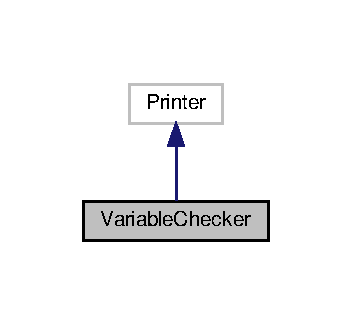
\includegraphics[width=169pt]{classVariableChecker__inherit__graph}
\end{center}
\end{figure}


Collaboration diagram for Variable\+Checker\+:\nopagebreak
\begin{figure}[H]
\begin{center}
\leavevmode
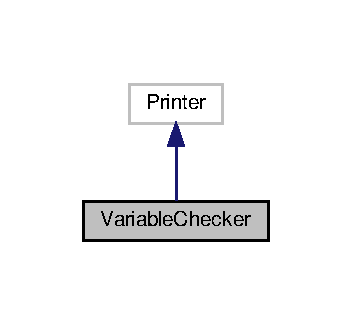
\includegraphics[width=169pt]{classVariableChecker__coll__graph}
\end{center}
\end{figure}
\subsection*{Public Member Functions}
\begin{DoxyCompactItemize}
\item 
\mbox{\Hypertarget{classVariableChecker_aae94b88c0d8cd1ed982c1104ff8a5620}\label{classVariableChecker_aae94b88c0d8cd1ed982c1104ff8a5620}} 
{\bfseries Variable\+Checker} (const \hyperlink{classVariableChecker}{Variable\+Checker} \&lv)=delete
\item 
\mbox{\Hypertarget{classVariableChecker_a176b4f4fadabfe1a2243433fd904d815}\label{classVariableChecker_a176b4f4fadabfe1a2243433fd904d815}} 
void {\bfseries Print\+C\+FG} (Function\+Decl $\ast$func)
\item 
\mbox{\Hypertarget{classVariableChecker_a9196341d6d8a0d80c045fc0d03d6f348}\label{classVariableChecker_a9196341d6d8a0d80c045fc0d03d6f348}} 
void {\bfseries Print\+Live\+Variables} (Function\+Decl $\ast$func)
\end{DoxyCompactItemize}


\subsection{Detailed Description}
工具类:活跃变量展示 

The documentation for this class was generated from the following files\+:\begin{DoxyCompactItemize}
\item 
/mnt/hgfs/\+Git\+Hub/\+S\+Eexperiement/backend/\+A\+S\+T\+Visitor/src/\+Slow\+Memory\+Checker/\hyperlink{VariableChecker_8h}{Variable\+Checker.\+h}\item 
/mnt/hgfs/\+Git\+Hub/\+S\+Eexperiement/backend/\+A\+S\+T\+Visitor/src/\+Slow\+Memory\+Checker/\hyperlink{VariableChecker_8cpp}{Variable\+Checker.\+cpp}\end{DoxyCompactItemize}

\chapter{File Documentation}
\hypertarget{readConfig_8h}{}\section{/mnt/hgfs/\+Git\+Hub/\+S\+Eexperiement/backend/\+A\+S\+T\+Visitor/src/\+Slow\+Memory\+Checker/read\+Config.h File Reference}
\label{readConfig_8h}\index{/mnt/hgfs/\+Git\+Hub/\+S\+Eexperiement/backend/\+A\+S\+T\+Visitor/src/\+Slow\+Memory\+Checker/read\+Config.\+h@{/mnt/hgfs/\+Git\+Hub/\+S\+Eexperiement/backend/\+A\+S\+T\+Visitor/src/\+Slow\+Memory\+Checker/read\+Config.\+h}}
{\ttfamily \#include $<$stdio.\+h$>$}\newline
{\ttfamily \#include $<$stdlib.\+h$>$}\newline
{\ttfamily \#include $<$string.\+h$>$}\newline
{\ttfamily \#include $<$assert.\+h$>$}\newline
{\ttfamily \#include $<$errno.\+h$>$}\newline
{\ttfamily \#include $<$ctype.\+h$>$}\newline
Include dependency graph for read\+Config.\+h\+:\nopagebreak
\begin{figure}[H]
\begin{center}
\leavevmode
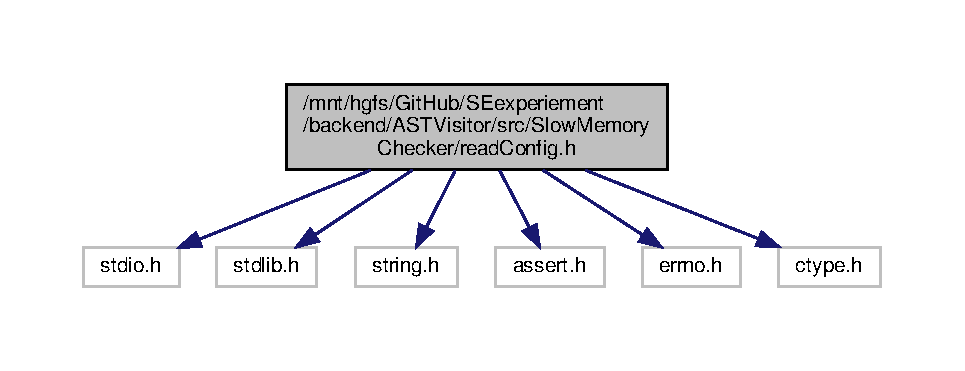
\includegraphics[width=350pt]{readConfig_8h__incl}
\end{center}
\end{figure}
This graph shows which files directly or indirectly include this file\+:\nopagebreak
\begin{figure}[H]
\begin{center}
\leavevmode
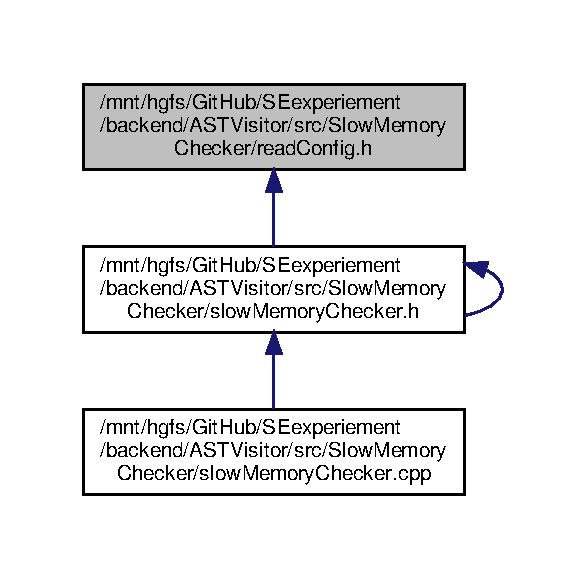
\includegraphics[width=281pt]{readConfig_8h__dep__incl}
\end{center}
\end{figure}
\subsection*{Classes}
\begin{DoxyCompactItemize}
\item 
class \hyperlink{classReadConfig}{Read\+Config}
\end{DoxyCompactItemize}
\subsection*{Macros}
\begin{DoxyCompactItemize}
\item 
\mbox{\Hypertarget{readConfig_8h_ab4189d6cdc71d0ac1445cf7f77aa68b2}\label{readConfig_8h_ab4189d6cdc71d0ac1445cf7f77aa68b2}} 
\#define {\bfseries K\+E\+Y\+V\+A\+L\+L\+EN}~100
\end{DoxyCompactItemize}


\subsection{Detailed Description}
\begin{DoxyAuthor}{Author}
叶宙果 
\end{DoxyAuthor}
\begin{DoxyVersion}{Version}
v2 
\end{DoxyVersion}

\hypertarget{slowMemoryChecker_8cpp}{}\section{/mnt/hgfs/\+Git\+Hub/\+S\+Eexperiement/backend/\+A\+S\+T\+Visitor/src/\+Slow\+Memory\+Checker/slow\+Memory\+Checker.cpp File Reference}
\label{slowMemoryChecker_8cpp}\index{/mnt/hgfs/\+Git\+Hub/\+S\+Eexperiement/backend/\+A\+S\+T\+Visitor/src/\+Slow\+Memory\+Checker/slow\+Memory\+Checker.\+cpp@{/mnt/hgfs/\+Git\+Hub/\+S\+Eexperiement/backend/\+A\+S\+T\+Visitor/src/\+Slow\+Memory\+Checker/slow\+Memory\+Checker.\+cpp}}
{\ttfamily \#include \char`\"{}slow\+Memory\+Checker.\+h\char`\"{}}\newline
Include dependency graph for slow\+Memory\+Checker.\+cpp\+:\nopagebreak
\begin{figure}[H]
\begin{center}
\leavevmode
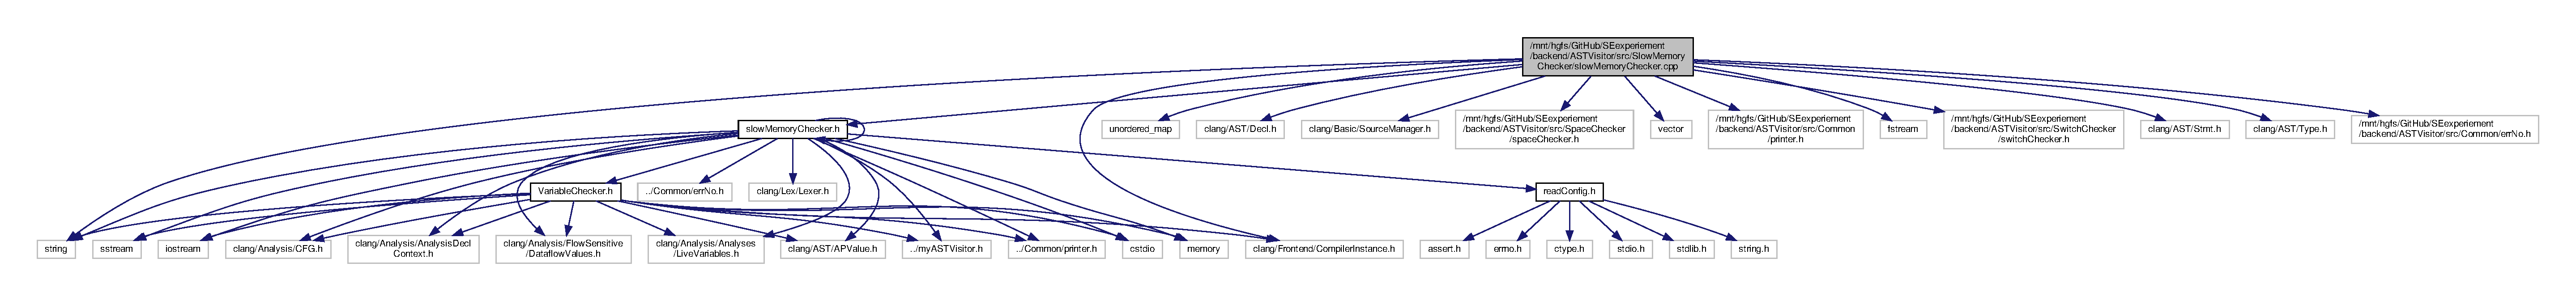
\includegraphics[width=350pt]{slowMemoryChecker_8cpp__incl}
\end{center}
\end{figure}


\subsection{Detailed Description}
\begin{DoxyAuthor}{Author}
叶宙果 
\end{DoxyAuthor}
\begin{DoxyVersion}{Version}
v2 
\end{DoxyVersion}

\hypertarget{slowMemoryChecker_8h}{}\section{/mnt/hgfs/\+Git\+Hub/\+S\+Eexperiement/backend/\+A\+S\+T\+Visitor/src/\+Slow\+Memory\+Checker/slow\+Memory\+Checker.h File Reference}
\label{slowMemoryChecker_8h}\index{/mnt/hgfs/\+Git\+Hub/\+S\+Eexperiement/backend/\+A\+S\+T\+Visitor/src/\+Slow\+Memory\+Checker/slow\+Memory\+Checker.\+h@{/mnt/hgfs/\+Git\+Hub/\+S\+Eexperiement/backend/\+A\+S\+T\+Visitor/src/\+Slow\+Memory\+Checker/slow\+Memory\+Checker.\+h}}
{\ttfamily \#include \char`\"{}../my\+A\+S\+T\+Visitor.\+h\char`\"{}}\newline
{\ttfamily \#include \char`\"{}../\+Common/printer.\+h\char`\"{}}\newline
{\ttfamily \#include \char`\"{}../\+Common/err\+No.\+h\char`\"{}}\newline
{\ttfamily \#include $<$cstdio$>$}\newline
{\ttfamily \#include $<$memory$>$}\newline
{\ttfamily \#include $<$sstream$>$}\newline
{\ttfamily \#include $<$string$>$}\newline
{\ttfamily \#include $<$iostream$>$}\newline
{\ttfamily \#include \char`\"{}clang/\+Lex/\+Lexer.\+h\char`\"{}}\newline
{\ttfamily \#include \char`\"{}clang/\+Analysis/\+C\+F\+G.\+h\char`\"{}}\newline
{\ttfamily \#include \char`\"{}clang/\+Analysis/\+Analysis\+Decl\+Context.\+h\char`\"{}}\newline
{\ttfamily \#include \char`\"{}clang/\+Analysis/\+Flow\+Sensitive/\+Dataflow\+Values.\+h\char`\"{}}\newline
{\ttfamily \#include \char`\"{}clang/\+Analysis/\+Analyses/\+Live\+Variables.\+h\char`\"{}}\newline
{\ttfamily \#include \char`\"{}clang/\+A\+S\+T/\+A\+P\+Value.\+h\char`\"{}}\newline
{\ttfamily \#include \char`\"{}slow\+Memory\+Checker.\+h\char`\"{}}\newline
{\ttfamily \#include \char`\"{}Variable\+Checker.\+h\char`\"{}}\newline
{\ttfamily \#include \char`\"{}read\+Config.\+h\char`\"{}}\newline
Include dependency graph for slow\+Memory\+Checker.\+h\+:\nopagebreak
\begin{figure}[H]
\begin{center}
\leavevmode
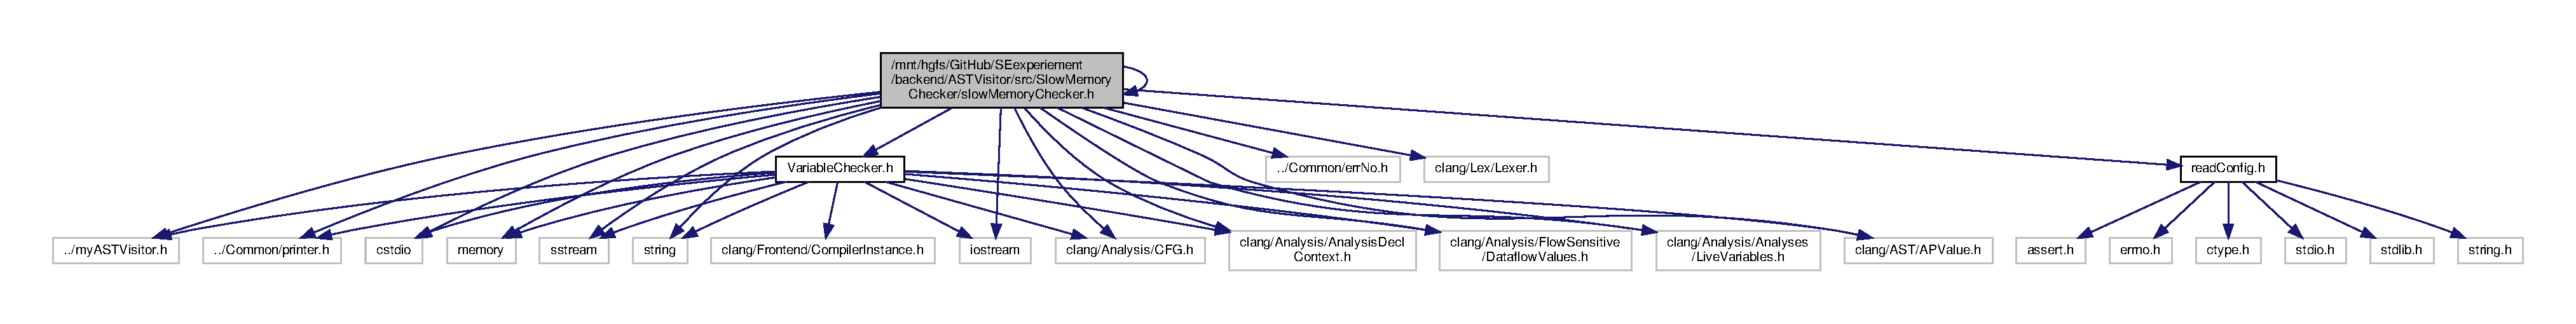
\includegraphics[width=350pt]{slowMemoryChecker_8h__incl}
\end{center}
\end{figure}
This graph shows which files directly or indirectly include this file\+:\nopagebreak
\begin{figure}[H]
\begin{center}
\leavevmode
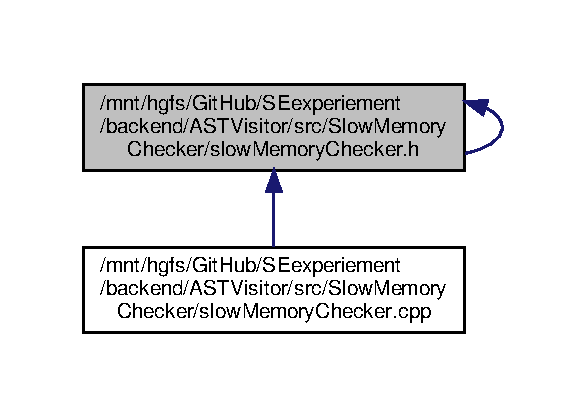
\includegraphics[width=281pt]{slowMemoryChecker_8h__dep__incl}
\end{center}
\end{figure}
\subsection*{Classes}
\begin{DoxyCompactItemize}
\item 
class \hyperlink{classForStmtCondLoc}{For\+Stmt\+Cond\+Loc}
\item 
class \hyperlink{classSlowMemoryChecker}{Slow\+Memory\+Checker}
\end{DoxyCompactItemize}


\subsection{Detailed Description}
\begin{DoxyAuthor}{Author}
叶宙果 
\end{DoxyAuthor}
\begin{DoxyVersion}{Version}
v2 
\end{DoxyVersion}

\hypertarget{VariableChecker_8cpp}{}\section{/mnt/hgfs/\+Git\+Hub/\+S\+Eexperiement/backend/\+A\+S\+T\+Visitor/src/\+Slow\+Memory\+Checker/\+Variable\+Checker.cpp File Reference}
\label{VariableChecker_8cpp}\index{/mnt/hgfs/\+Git\+Hub/\+S\+Eexperiement/backend/\+A\+S\+T\+Visitor/src/\+Slow\+Memory\+Checker/\+Variable\+Checker.\+cpp@{/mnt/hgfs/\+Git\+Hub/\+S\+Eexperiement/backend/\+A\+S\+T\+Visitor/src/\+Slow\+Memory\+Checker/\+Variable\+Checker.\+cpp}}
{\ttfamily \#include \char`\"{}Variable\+Checker.\+h\char`\"{}}\newline
Include dependency graph for Variable\+Checker.\+cpp\+:\nopagebreak
\begin{figure}[H]
\begin{center}
\leavevmode
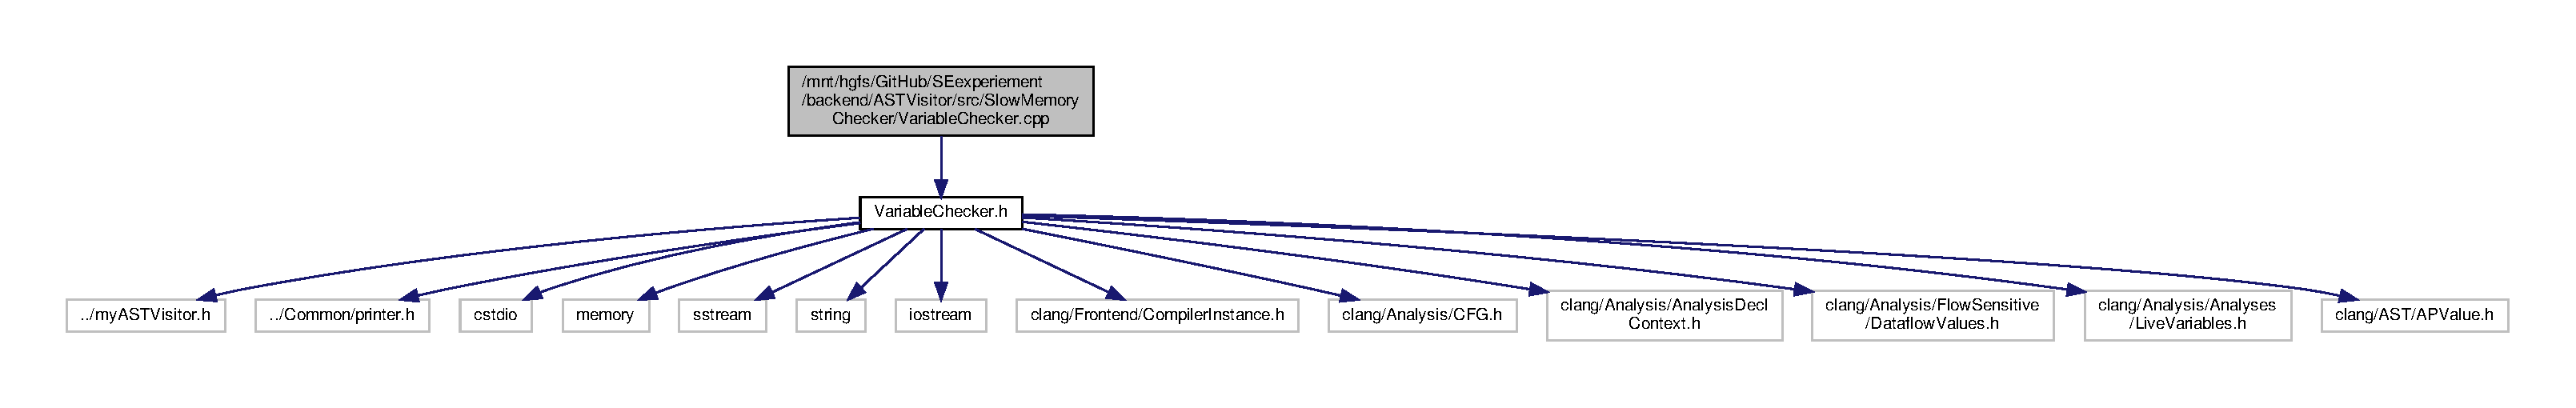
\includegraphics[width=350pt]{VariableChecker_8cpp__incl}
\end{center}
\end{figure}


\subsection{Detailed Description}
\begin{DoxyAuthor}{Author}
叶宙果 
\end{DoxyAuthor}
\begin{DoxyVersion}{Version}
v2 
\end{DoxyVersion}

\hypertarget{VariableChecker_8h}{}\section{/mnt/hgfs/\+Git\+Hub/\+S\+Eexperiement/backend/\+A\+S\+T\+Visitor/src/\+Slow\+Memory\+Checker/\+Variable\+Checker.h File Reference}
\label{VariableChecker_8h}\index{/mnt/hgfs/\+Git\+Hub/\+S\+Eexperiement/backend/\+A\+S\+T\+Visitor/src/\+Slow\+Memory\+Checker/\+Variable\+Checker.\+h@{/mnt/hgfs/\+Git\+Hub/\+S\+Eexperiement/backend/\+A\+S\+T\+Visitor/src/\+Slow\+Memory\+Checker/\+Variable\+Checker.\+h}}
{\ttfamily \#include \char`\"{}../my\+A\+S\+T\+Visitor.\+h\char`\"{}}\newline
{\ttfamily \#include \char`\"{}../\+Common/printer.\+h\char`\"{}}\newline
{\ttfamily \#include $<$cstdio$>$}\newline
{\ttfamily \#include $<$memory$>$}\newline
{\ttfamily \#include $<$sstream$>$}\newline
{\ttfamily \#include $<$string$>$}\newline
{\ttfamily \#include $<$iostream$>$}\newline
{\ttfamily \#include \char`\"{}clang/\+Frontend/\+Compiler\+Instance.\+h\char`\"{}}\newline
{\ttfamily \#include \char`\"{}clang/\+Analysis/\+C\+F\+G.\+h\char`\"{}}\newline
{\ttfamily \#include \char`\"{}clang/\+Analysis/\+Analysis\+Decl\+Context.\+h\char`\"{}}\newline
{\ttfamily \#include \char`\"{}clang/\+Analysis/\+Flow\+Sensitive/\+Dataflow\+Values.\+h\char`\"{}}\newline
{\ttfamily \#include \char`\"{}clang/\+Analysis/\+Analyses/\+Live\+Variables.\+h\char`\"{}}\newline
{\ttfamily \#include \char`\"{}clang/\+A\+S\+T/\+A\+P\+Value.\+h\char`\"{}}\newline
Include dependency graph for Variable\+Checker.\+h\+:\nopagebreak
\begin{figure}[H]
\begin{center}
\leavevmode
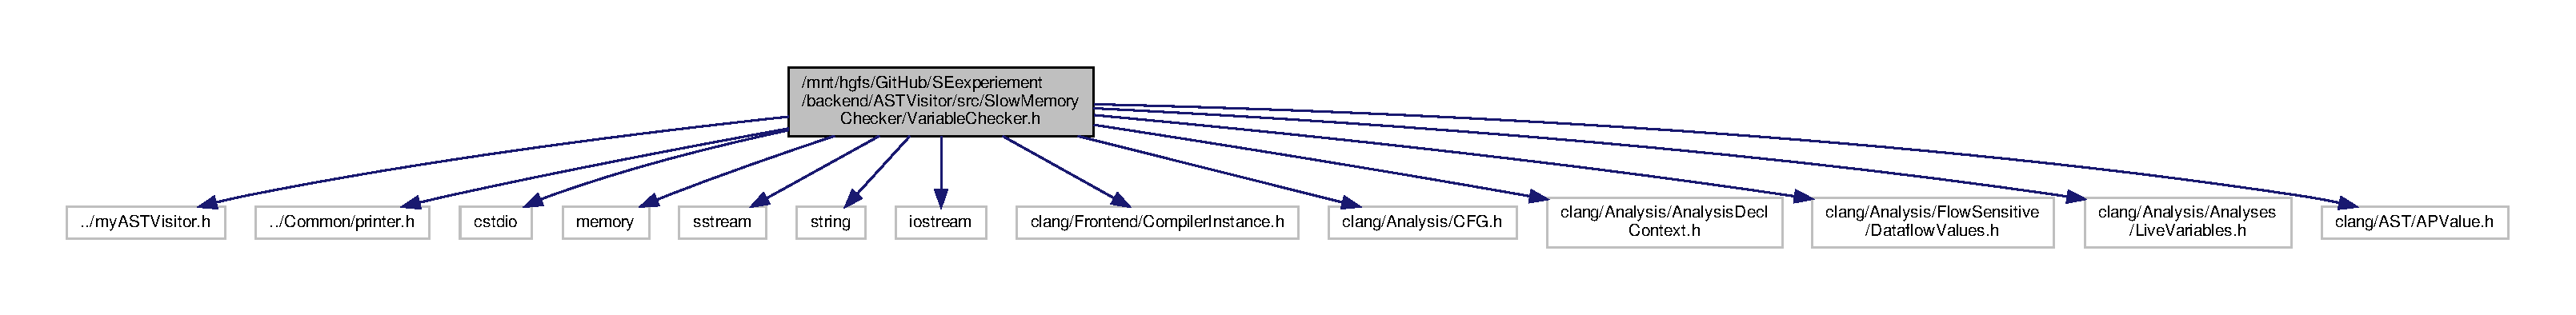
\includegraphics[width=350pt]{VariableChecker_8h__incl}
\end{center}
\end{figure}
This graph shows which files directly or indirectly include this file\+:\nopagebreak
\begin{figure}[H]
\begin{center}
\leavevmode
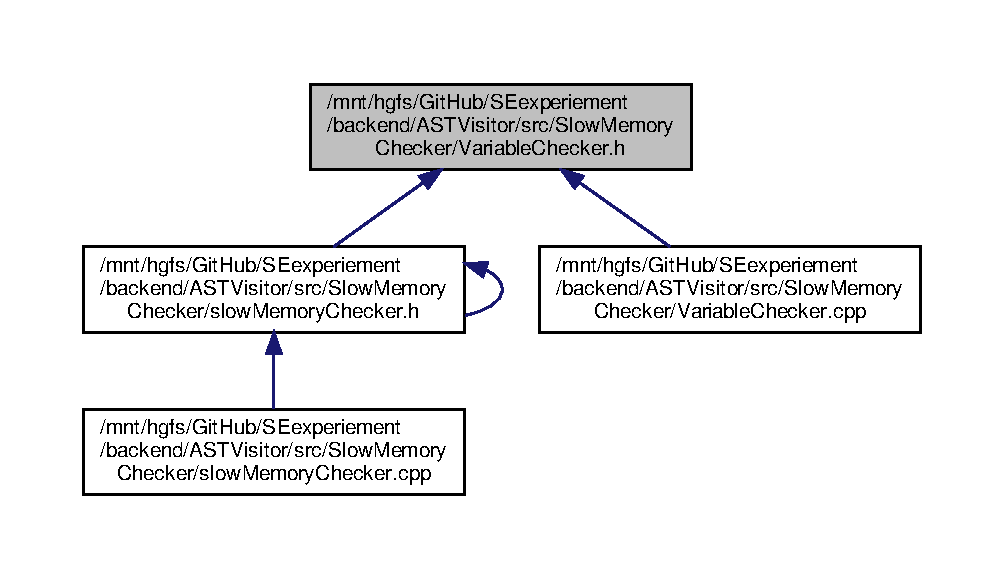
\includegraphics[width=350pt]{VariableChecker_8h__dep__incl}
\end{center}
\end{figure}
\subsection*{Classes}
\begin{DoxyCompactItemize}
\item 
class \hyperlink{classVariableChecker}{Variable\+Checker}
\end{DoxyCompactItemize}


\subsection{Detailed Description}
\begin{DoxyAuthor}{Author}
叶宙果 
\end{DoxyAuthor}
\begin{DoxyVersion}{Version}
v2 
\end{DoxyVersion}

%--- End generated contents ---

% Index
\backmatter
\newpage
\phantomsection
\clearemptydoublepage
\addcontentsline{toc}{chapter}{Index}
\printindex

\end{document}
